\documentclass{article}\usepackage[]{graphicx}\usepackage[]{color}
% maxwidth is the original width if it is less than linewidth
% otherwise use linewidth (to make sure the graphics do not exceed the margin)
\makeatletter
\def\maxwidth{ %
  \ifdim\Gin@nat@width>\linewidth
    \linewidth
  \else
    \Gin@nat@width
  \fi
}
\makeatother

\definecolor{fgcolor}{rgb}{0.196, 0.196, 0.196}
\newcommand{\hlnum}[1]{\textcolor[rgb]{0.063,0.58,0.627}{#1}}%
\newcommand{\hlstr}[1]{\textcolor[rgb]{0.063,0.58,0.627}{#1}}%
\newcommand{\hlcom}[1]{\textcolor[rgb]{0.588,0.588,0.588}{#1}}%
\newcommand{\hlopt}[1]{\textcolor[rgb]{0.196,0.196,0.196}{#1}}%
\newcommand{\hlstd}[1]{\textcolor[rgb]{0.196,0.196,0.196}{#1}}%
\newcommand{\hlkwa}[1]{\textcolor[rgb]{0.231,0.416,0.784}{#1}}%
\newcommand{\hlkwb}[1]{\textcolor[rgb]{0.627,0,0.314}{#1}}%
\newcommand{\hlkwc}[1]{\textcolor[rgb]{0,0.631,0.314}{#1}}%
\newcommand{\hlkwd}[1]{\textcolor[rgb]{0.78,0.227,0.412}{#1}}%
\let\hlipl\hlkwb

\usepackage{framed}
\makeatletter
\newenvironment{kframe}{%
 \def\at@end@of@kframe{}%
 \ifinner\ifhmode%
  \def\at@end@of@kframe{\end{minipage}}%
  \begin{minipage}{\columnwidth}%
 \fi\fi%
 \def\FrameCommand##1{\hskip\@totalleftmargin \hskip-\fboxsep
 \colorbox{shadecolor}{##1}\hskip-\fboxsep
     % There is no \\@totalrightmargin, so:
     \hskip-\linewidth \hskip-\@totalleftmargin \hskip\columnwidth}%
 \MakeFramed {\advance\hsize-\width
   \@totalleftmargin\z@ \linewidth\hsize
   \@setminipage}}%
 {\par\unskip\endMakeFramed%
 \at@end@of@kframe}
\makeatother

\definecolor{shadecolor}{rgb}{.97, .97, .97}
\definecolor{messagecolor}{rgb}{0, 0, 0}
\definecolor{warningcolor}{rgb}{1, 0, 1}
\definecolor{errorcolor}{rgb}{1, 0, 0}
\newenvironment{knitrout}{}{} % an empty environment to be redefined in TeX

\usepackage{alltt}
\usepackage{fullpage}
\usepackage{mathtools}
\usepackage{amsmath,amsthm,amssymb}
\usepackage{graphicx}
\usepackage[dvipsnames]{xcolor}
\usepackage{float}
\usepackage{caption}
\usepackage{wrapfig}
\usepackage{multicol}
\usepackage{multirow}
\usepackage{booktabs}
\usepackage{bm}
\usepackage{enumitem}
\usepackage{authblk}
\usepackage{rotating}
\usepackage{array}
\usepackage{colortbl}
\usepackage{siunitx}
\usepackage{authblk}
\sisetup{output-exponent-marker=\ensuremath{\mathrm{e}}}

%% Supplemental figure notation
\renewcommand\thefigure{S\arabic{figure}}
\renewcommand\thetable{S\arabic{table}}

\DeclareUnicodeCharacter{251C}{\mbox{\kern.23em
  \vrule height2.2exdepth1exwidth.4pt\vrule height2.2ptdepth-1.8ptwidth.23em}}
\DeclareUnicodeCharacter{2500}{\mbox{\vrule height2.2ptdepth-1.8ptwidth.5em}}
\DeclareUnicodeCharacter{2514}{\mbox{\kern.23em
  \vrule height2.2exdepth-1.8ptwidth.4pt\vrule height2.2ptdepth-1.8ptwidth.23em}}
\DeclareUnicodeCharacter{2052}{\textdiscount}

\setlength{\parindent}{0em}
\setlength{\parskip}{1ex}
\IfFileExists{upquote.sty}{\usepackage{upquote}}{}
\begin{document}



\title{Pre-capture multiplexing provides additional power to detect copy number variation in exome sequencing: Supplemental Information}
\author[1,2]{Dayne L. Filer}
\author[1]{Fengshen Kuo}
\author[1]{Alicia T. Brandt}
\author[1]{Christian R. Tilley}
\author[1]{Piotr A. Mieczkowski}
\author[1]{Jonathan S. Berg}
\author[1,2,3]{Kimberly Robasky}
\author[1,4]{Yun Li}
\author[2]{Chris Bizon}
\author[2]{Jeffery L. Tilson}
\author[1,2]{Bradford C. Powell}
\author[1,2]{Darius M. Bost}
\author[2]{Clark D. Jeffries}
\author[1,2,5]{Kirk C. Wilhelmsen}
\affil[1]{Department of Genetics, UNC School of Medicine, Chapel Hill, NC}
\affil[2]{Renaissance Computing Institute, Chapel Hill, NC}
\affil[3]{UNC School of Information and Library Science, Chapel Hill, NC}
\affil[4]{Department of Biostatistics, UNC Gillings School of Global Public Health, Chapel Hill, NC}
\affil[5]{Department of Neurology, UNC School of Medicine, Chapel Hill, NC}

\date{}

\maketitle

\tableofcontents

\newpage
\section{Setup}

\begin{knitrout}
\definecolor{shadecolor}{rgb}{0.969, 0.969, 0.969}\color{fgcolor}\begin{kframe}
\begin{alltt}
\hlkwd{library}\hlstd{(filer2020A)}
\hlkwd{library}\hlstd{(mcCNV)}
\hlkwd{library}\hlstd{(eulerr)}
\hlkwd{library}\hlstd{(dlfUtils)}
\hlkwd{library}\hlstd{(parallel)}
\hlkwd{library}\hlstd{(grid)}
\end{alltt}
\end{kframe}
\end{knitrout}

\section{Summary of data}

\begin{knitrout}
\definecolor{shadecolor}{rgb}{0.969, 0.969, 0.969}\color{fgcolor}\begin{kframe}
\begin{alltt}
\hlkwd{data}\hlstd{(subjectMeta)}
\hlstd{poolTbl} \hlkwb{<-} \hlstd{subjectMeta[ ,}
                       \hlkwd{.}\hlstd{(}\hlkwc{N} \hlstd{= .N,}
                         \hlkwc{medExon} \hlstd{=} \hlkwd{round}\hlstd{(}\hlkwd{median}\hlstd{(medIntMolCount),} \hlnum{0}\hlstd{),}
                         \hlkwc{medTotal} \hlstd{=} \hlkwd{round}\hlstd{(}\hlkwd{median}\hlstd{(totalMolCount),} \hlnum{0}\hlstd{),}
                         \hlkwc{minTotal} \hlstd{=} \hlkwd{min}\hlstd{(totalMolCount),}
                         \hlkwc{maxTotal} \hlstd{=} \hlkwd{max}\hlstd{(totalMolCount),}
                         \hlkwc{rsdTotal} \hlstd{=} \hlkwd{sd}\hlstd{(totalMolCount)}\hlopt{/}\hlkwd{mean}\hlstd{(totalMolCount)}\hlopt{*}\hlnum{100}\hlstd{),}
                       \hlkwc{by} \hlstd{=} \hlkwd{.}\hlstd{(pool, capture, multiplexCapture)]}
\hlstd{poolTbl[ , rsdTotal} \hlkwb{:=} \hlkwd{round}\hlstd{(rsdTotal,} \hlnum{1}\hlstd{)]}
\hlstd{poolTbl}
\end{alltt}
\begin{verbatim}
##       pool capture multiplexCapture   N medExon medTotal minTotal  maxTotal
## 1:  IDT-IC     IDT            FALSE  16     143 55149058 37453015  85138915
## 2:  IDT-MC     IDT             TRUE  16      93 29772684 16674468 118147912
## 3:  IDT-RR     IDT             TRUE  16     272 79079629 61289322 120147888
## 4: NCGENES Agilent            FALSE 112      93 24451245 12749793  68565471
## 5:   Pool1 Agilent             TRUE  16      56 13265614  8911132  17324903
## 6:   Pool2 Agilent             TRUE  16      86 21076056  4585195  27846146
## 7:    SMA1 Agilent             TRUE   8      56 12256002 11051840  13600697
## 8:    SMA2 Agilent             TRUE   8      25  5622040  4904000   6545360
## 9:     WGS Agilent             TRUE  16     196 46406224 36496097  65200410
##    rsdTotal
## 1:     22.4
## 2:     64.2
## 3:     22.9
## 4:     27.6
## 5:     18.5
## 6:     27.6
## 7:      6.2
## 8:     10.4
## 9:     16.4
\end{verbatim}
\end{kframe}
\end{knitrout}

\newpage
\section{Mean-variance relationship for multplexed versus independent capture}

To show the difference in independent and multiplexed captures, we randomly select pools of samples independently-captured using the same platform.
We then calculate interval statistics (mean, variance, etc.) across the pools.
\begin{knitrout}
\definecolor{shadecolor}{rgb}{0.969, 0.969, 0.969}\color{fgcolor}\begin{kframe}
\begin{alltt}
\hlstd{smplSubject} \hlkwb{<-} \hlkwa{function}\hlstd{(}\hlkwc{poolName}\hlstd{,} \hlkwc{n}\hlstd{) \{}
  \hlkwd{data}\hlstd{(subjectMeta,} \hlkwc{envir} \hlstd{=} \hlkwd{environment}\hlstd{())}
  \hlstd{subjectMeta[pool} \hlopt{==} \hlstd{poolName,} \hlkwd{sample}\hlstd{(subject, n,} \hlkwc{replace} \hlstd{=} \hlnum{FALSE}\hlstd{)]}
\hlstd{\}}
\hlkwd{set.seed}\hlstd{(}\hlnum{1234}\hlstd{)}
\hlstd{pools} \hlkwb{<-} \hlkwd{c}\hlstd{(}\hlkwd{replicate}\hlstd{(}\hlnum{5}\hlstd{,} \hlkwd{smplSubject}\hlstd{(}\hlstr{"NCGENES"}\hlstd{,} \hlnum{16}\hlstd{),} \hlkwc{simplify} \hlstd{=} \hlnum{FALSE}\hlstd{))}
\hlkwd{names}\hlstd{(pools)} \hlkwb{<-} \hlkwd{c}\hlstd{(}\hlkwd{sprintf}\hlstd{(}\hlstr{"randNCG_%d"}\hlstd{,} \hlnum{1}\hlopt{:}\hlnum{5}\hlstd{))}
\hlstd{pools} \hlkwb{<-} \hlkwd{c}\hlstd{(pools,}
           \hlkwd{with}\hlstd{(subjectMeta[pool} \hlopt{!=} \hlstr{"NCGENES"}\hlstd{],} \hlkwd{split}\hlstd{(subject, pool)))}
\end{alltt}
\end{kframe}
\end{knitrout}

\begin{knitrout}
\definecolor{shadecolor}{rgb}{0.969, 0.969, 0.969}\color{fgcolor}\begin{kframe}
\begin{alltt}
\hlcom{## Calculate mean-variance by pool}
\hlstd{mnvr} \hlkwb{<-} \hlkwd{mclapply}\hlstd{(pools, subsetCounts,} \hlkwc{mc.cores} \hlstd{=} \hlkwd{length}\hlstd{(pools))}
\hlstd{mnvr} \hlkwb{<-} \hlkwd{mclapply}\hlstd{(mnvr, calcIntStats,} \hlkwc{mc.cores} \hlstd{=} \hlkwd{length}\hlstd{(mnvr))}
\hlkwa{for} \hlstd{(i} \hlkwa{in} \hlkwd{seq_along}\hlstd{(mnvr)) \{}
  \hlstd{mnvr[[i]][ , pool} \hlkwb{:=} \hlkwd{names}\hlstd{(mnvr)[i]]}
\hlstd{\}}
\hlstd{mnvr} \hlkwb{<-} \hlkwd{rbindlist}\hlstd{(mnvr)}
\hlkwd{setkey}\hlstd{(mnvr, pool);} \hlkwd{setcolorder}\hlstd{(mnvr)}

\hlcom{## Estimate alpha0}
\hlstd{alpha0} \hlkwb{<-} \hlkwd{mclapply}\hlstd{(pools, estAlpha0,} \hlkwc{mc.cores} \hlstd{=} \hlkwd{length}\hlstd{(pools))}
\end{alltt}
\end{kframe}
\end{knitrout}

\begin{knitrout}
\definecolor{shadecolor}{rgb}{0.969, 0.969, 0.969}\color{fgcolor}\begin{kframe}
\begin{alltt}
\hlstd{a0tbl} \hlkwb{<-} \hlkwd{data.table}\hlstd{(}\hlkwc{pool} \hlstd{=} \hlkwd{names}\hlstd{(alpha0),}
                    \hlkwc{a0} \hlstd{=} \hlkwd{sapply}\hlstd{(alpha0,} \hlstr{"[["}\hlstd{,} \hlstr{"a0"}\hlstd{),}
                    \hlkwc{N} \hlstd{=} \hlkwd{sapply}\hlstd{(alpha0,} \hlstr{"[["}\hlstd{,} \hlstr{"N"}\hlstd{))}
\hlstd{a0tbl[ , aMn} \hlkwb{:=} \hlstd{a0}\hlopt{/}\hlstd{N]}
\hlstd{calcRange} \hlkwb{<-} \hlkwa{function}\hlstd{(}\hlkwc{x}\hlstd{) \{}
  \hlstd{subjectMeta[subject} \hlopt \hlstd{x,}
              \hlkwd{.}\hlstd{(}\hlkwc{mnCount} \hlstd{=} \hlkwd{min}\hlstd{(totalMolCount),}
                \hlkwc{mdCount} \hlstd{=} \hlkwd{median}\hlstd{(totalMolCount),}
                \hlkwc{mxCount} \hlstd{=} \hlkwd{max}\hlstd{(totalMolCount),}
                \hlkwc{rsCount} \hlstd{=} \hlkwd{sd}\hlstd{(totalMolCount)}\hlopt{/}\hlkwd{mean}\hlstd{(totalMolCount)}\hlopt{*}\hlnum{100}\hlstd{)]}
\hlstd{\}}
\hlstd{poolCts} \hlkwb{<-} \hlkwd{lapply}\hlstd{(pools, calcRange)}
\hlstd{poolCts} \hlkwb{<-} \hlkwd{lapply}\hlstd{(}\hlkwd{names}\hlstd{(poolCts),} \hlkwa{function}\hlstd{(}\hlkwc{x}\hlstd{) poolCts[[x]][ , pool} \hlkwb{:=} \hlstd{x])}
\hlstd{poolCts} \hlkwb{<-} \hlkwd{rbindlist}\hlstd{(poolCts)}
\hlstd{a0tbl} \hlkwb{<-} \hlkwd{merge}\hlstd{(a0tbl, poolCts)}
\hlstd{a0tbl[ , mc} \hlkwb{:=} \hlopt{!}\hlkwd{grepl}\hlstd{(}\hlstr{"IDT-IC|rand"}\hlstd{, pool)]}
\hlstd{a0tbl[ , idt} \hlkwb{:=} \hlkwd{grepl}\hlstd{(}\hlstr{"IDT"}\hlstd{, pool)]}
\end{alltt}
\end{kframe}
\end{knitrout}

\begin{knitrout}
\definecolor{shadecolor}{rgb}{0.969, 0.969, 0.969}\color{fgcolor}\begin{kframe}
\begin{alltt}
\hlkwd{pltAlpha0}\hlstd{(a0tbl)}
\end{alltt}
\end{kframe}
\end{knitrout}

\begin{figure}[H]
  \centering
  \includegraphics[]{figures-a0plot-1.pdf}
  \caption{manuscript figure}
\end{figure}

\newpage
\begin{knitrout}
\definecolor{shadecolor}{rgb}{0.969, 0.969, 0.969}\color{fgcolor}\begin{kframe}
\begin{alltt}
\hlstd{aglPools} \hlkwb{<-} \hlkwd{c}\hlstd{(}\hlkwd{sprintf}\hlstd{(}\hlstr{"randNCG_%d"}\hlstd{,} \hlnum{1}\hlopt{:}\hlnum{5}\hlstd{),} \hlstr{"Pool1"}\hlstd{,} \hlstr{"Pool2"}\hlstd{,} \hlstr{"WGS"}\hlstd{,} \hlstr{"SMA1"}\hlstd{,} \hlstr{"SMA2"}\hlstd{)}
\hlkwd{with}\hlstd{(mnvr[pool} \hlopt \hlstd{aglPools], \{}
  \hlkwd{pltMnVrCont}\hlstd{(}\hlkwc{dat} \hlstd{=} \hlkwd{as.data.table}\hlstd{(}\hlkwd{as.list}\hlstd{(}\hlkwd{environment}\hlstd{())),}
              \hlkwc{grpVec} \hlstd{=} \hlkwd{factor}\hlstd{(pool,} \hlkwc{levels} \hlstd{= aglPools),}
              \hlkwc{colVec} \hlstd{=} \hlkwd{c}\hlstd{(}\hlkwd{rep}\hlstd{(}\hlstr{'darkblue'}\hlstd{,} \hlnum{5}\hlstd{),} \hlkwd{rep}\hlstd{(}\hlstr{'darkorange'}\hlstd{,} \hlnum{5}\hlstd{)),}
              \hlkwc{lgnd} \hlstd{=} \hlnum{FALSE}\hlstd{)}
\hlstd{\})}
\hlkwd{addfiglab}\hlstd{(}\hlstr{"A"}\hlstd{,} \hlkwc{units} \hlstd{=} \hlstr{"ndc"}\hlstd{)}
\hlkwd{legend}\hlstd{(}\hlkwc{x} \hlstd{=} \hlstr{"center"}\hlstd{,} \hlkwc{lwd} \hlstd{=} \hlnum{4}\hlstd{,} \hlkwc{col} \hlstd{=} \hlkwd{c}\hlstd{(}\hlstr{'darkblue'}\hlstd{,} \hlstr{'darkorange'}\hlstd{),}
       \hlkwd{c}\hlstd{(}\hlstr{"AGL-IC"}\hlstd{,} \hlstr{"AGL-MC"}\hlstd{),} \hlkwc{bty} \hlstd{=} \hlstr{"n"}\hlstd{,} \hlkwc{cex} \hlstd{=} \hlnum{0.75}\hlstd{)}
\hlstd{idtPools} \hlkwb{<-} \hlkwd{c}\hlstd{(}\hlstr{"IDT-MC"}\hlstd{,} \hlstr{"IDT-IC"}\hlstd{,} \hlstr{"IDT-RR"}\hlstd{)}
\hlkwd{with}\hlstd{(mnvr[pool} \hlopt \hlstd{idtPools], \{}
  \hlkwd{pltMnVrCont}\hlstd{(}\hlkwc{dat} \hlstd{=} \hlkwd{as.data.table}\hlstd{(}\hlkwd{as.list}\hlstd{(}\hlkwd{environment}\hlstd{())),}
              \hlkwc{grpVec} \hlstd{=} \hlkwd{factor}\hlstd{(pool,} \hlkwc{levels} \hlstd{= idtPools),}
              \hlkwc{colVec} \hlstd{=} \hlkwd{c}\hlstd{(}\hlstr{"darkorange"}\hlstd{,} \hlstr{"darkblue"}\hlstd{,} \hlstr{"darkorange"}\hlstd{),}
              \hlkwc{lgnd} \hlstd{=} \hlnum{FALSE}\hlstd{)}
\hlstd{\})}
\hlkwd{addfiglab}\hlstd{(}\hlstr{"B"}\hlstd{)}
\hlkwd{legend}\hlstd{(}\hlkwc{x} \hlstd{=} \hlstr{"center"}\hlstd{,} \hlkwc{lwd} \hlstd{=} \hlnum{4}\hlstd{,} \hlkwc{col} \hlstd{=} \hlkwd{c}\hlstd{(}\hlstr{'darkblue'}\hlstd{,} \hlstr{'darkorange'}\hlstd{),}
       \hlkwd{c}\hlstd{(}\hlstr{"IDT-IC"}\hlstd{,} \hlstr{"IDT-MC"}\hlstd{),} \hlkwc{bty} \hlstd{=} \hlstr{"n"}\hlstd{,} \hlkwc{cex} \hlstd{=} \hlnum{0.75}\hlstd{)}
\hlkwd{with}\hlstd{(mnvr[pool} \hlopt \hlkwd{c}\hlstd{(}\hlstr{"WGS"}\hlstd{,} \hlstr{"IDT-RR"}\hlstd{)], \{}
  \hlkwd{pltMnVrCont}\hlstd{(}\hlkwc{dat} \hlstd{=} \hlkwd{as.data.table}\hlstd{(}\hlkwd{as.list}\hlstd{(}\hlkwd{environment}\hlstd{())),}
              \hlkwc{grpVec} \hlstd{=} \hlkwd{factor}\hlstd{(pool,} \hlkwc{levels} \hlstd{=} \hlkwd{c}\hlstd{(}\hlstr{"WGS"}\hlstd{,} \hlstr{"IDT-RR"}\hlstd{)),}
              \hlkwc{colVec} \hlstd{=} \hlkwd{c}\hlstd{(}\hlstr{"darkblue"}\hlstd{,} \hlstr{"darkorange"}\hlstd{))}
\hlstd{\})}
\end{alltt}
\end{kframe}
\end{knitrout}

\begin{figure}[H]
  \centering
  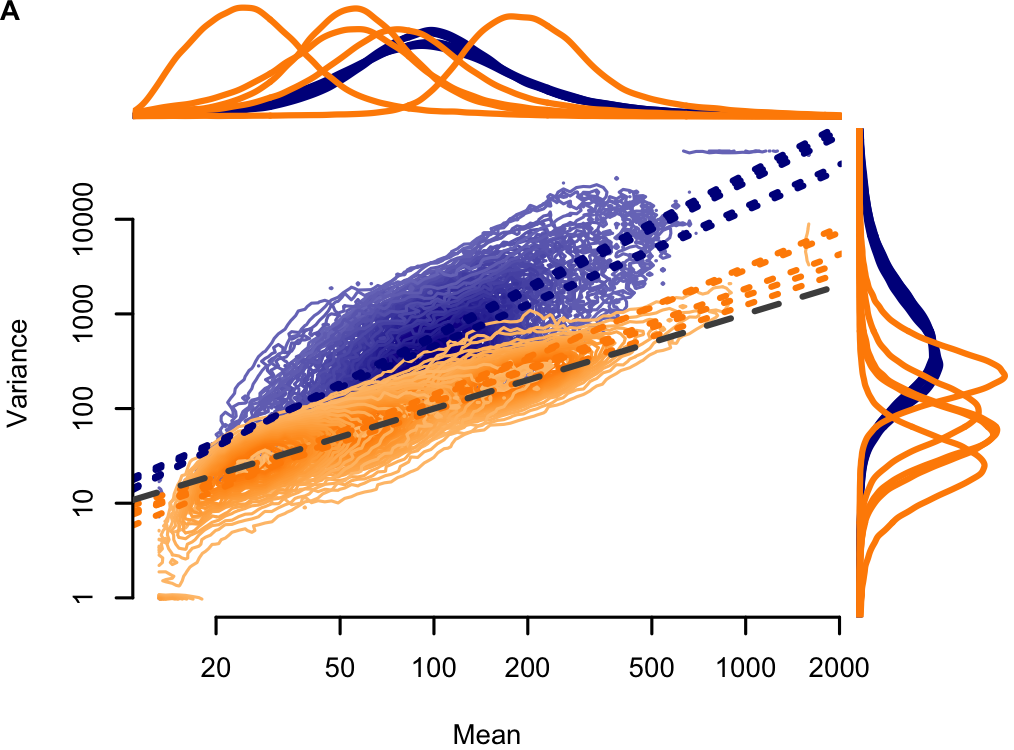
\includegraphics[]{figures-mnVrPlot-1.pdf}%
  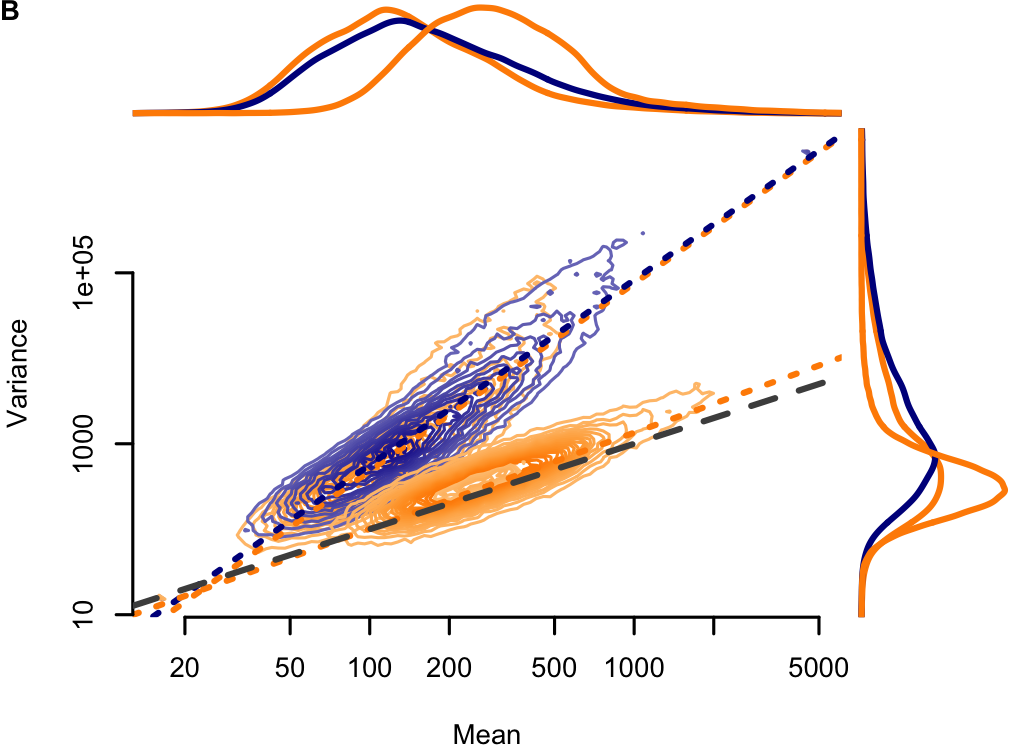
\includegraphics[]{figures-mnVrPlot-2.pdf}
  \caption{manuscript figure}
\end{figure}

\begin{figure}[H]
  \centering
  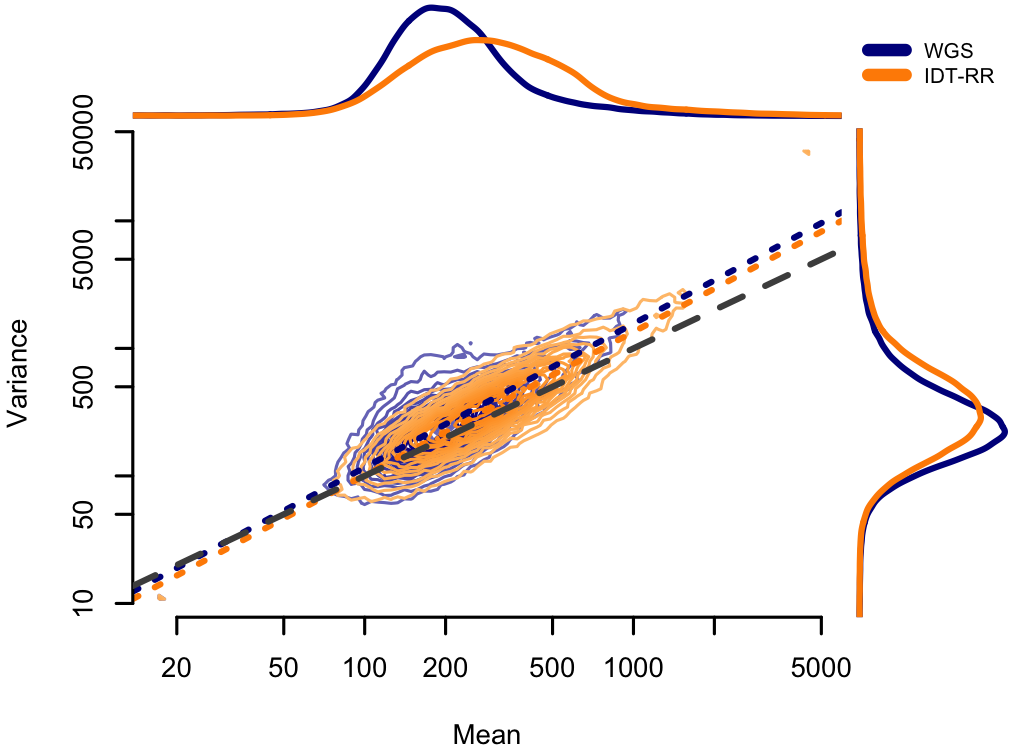
\includegraphics[]{figures-mnVrPlot-3.pdf}%
  \caption{Comparison of mean-variance relationship between WGS pool (blue) and IDT-RR pool (orange). Mean count by exon given on horizontal axis; variance of exon counts given on horizontal axis. Dotted lines show the ordinary least-squares fit. Lines above plot show the distribution of mean values; lines to the right of the plot show the distribution of variance values.}
\end{figure}

\newpage
\section{ExomeDepth selection}

\begin{knitrout}
\definecolor{shadecolor}{rgb}{0.969, 0.969, 0.969}\color{fgcolor}\begin{kframe}
\begin{alltt}
\hlkwd{pltSubjectStatByPool}\hlstd{(}\hlstr{"medIntMolCount"}\hlstd{,} \hlkwc{ylab} \hlstd{=} \hlstr{"Median count per exon"}\hlstd{)}
\hlkwd{addfiglab}\hlstd{(}\hlstr{"A"}\hlstd{)}
\hlkwd{pltSubjectStatByPool}\hlstd{(}\hlstr{"overallPhi"}\hlstd{,} \hlkwc{ylab} \hlstd{=} \hlstr{"Overdispersion (phi)"}\hlstd{)}
\hlkwd{addfiglab}\hlstd{(}\hlstr{"B"}\hlstd{)}
\hlkwd{pltSubjectStatByPool}\hlstd{(}\hlstr{"propSelected"}\hlstd{,} \hlkwc{ylab} \hlstd{=} \hlstr{"Proportion of controls selected"}\hlstd{)}
\hlkwd{addfiglab}\hlstd{(}\hlstr{"C"}\hlstd{)}
\hlkwd{pltSubjectStatByPool}\hlstd{(}\hlstr{"nSelected"}\hlstd{,} \hlkwc{ylab} \hlstd{=} \hlstr{"Number of controls selected"}\hlstd{)}
\hlkwd{addfiglab}\hlstd{(}\hlstr{"D"}\hlstd{)}
\end{alltt}
\end{kframe}
\end{knitrout}

\begin{figure}[H]
  \centering
  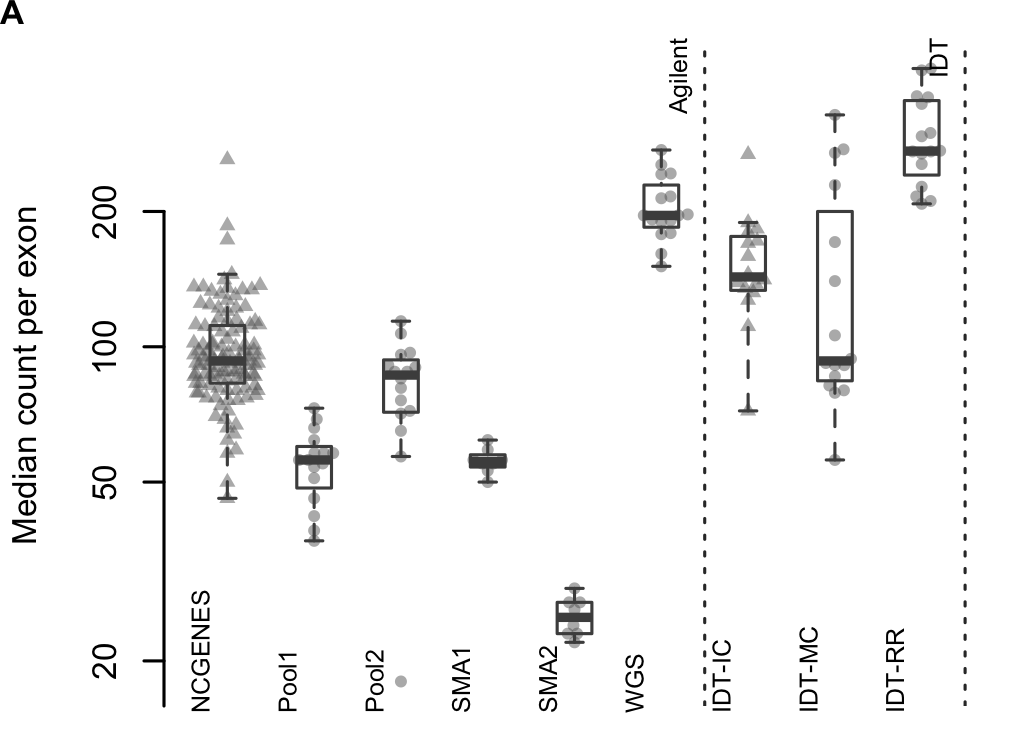
\includegraphics[]{figures-edSelection-1.pdf}%
  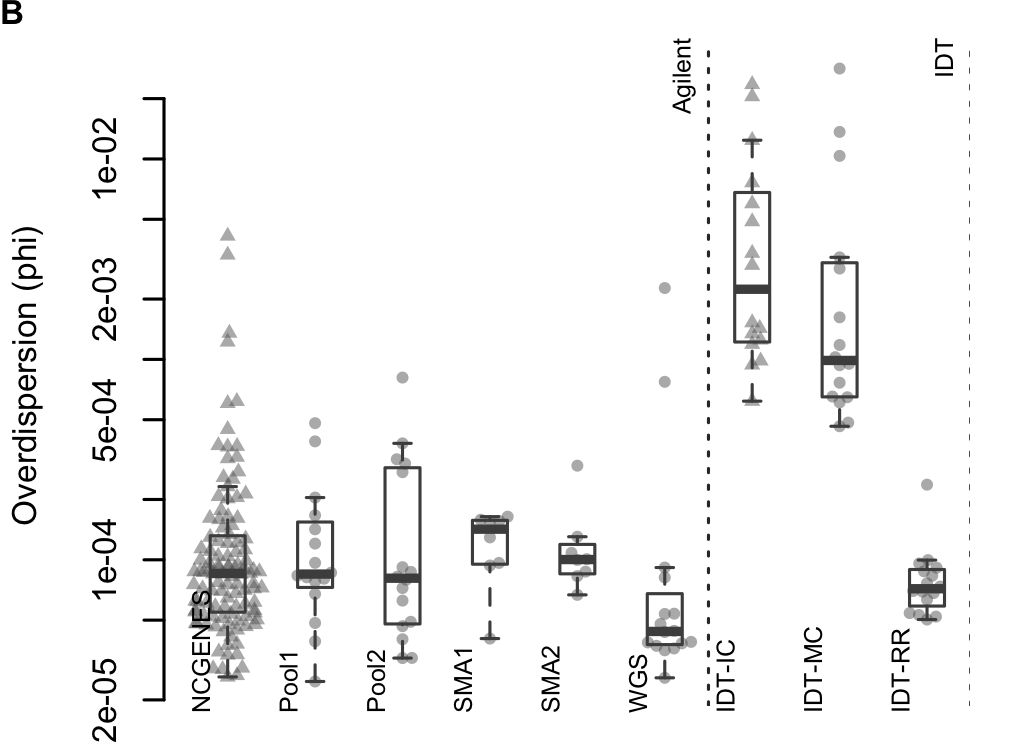
\includegraphics[]{figures-edSelection-2.pdf}
  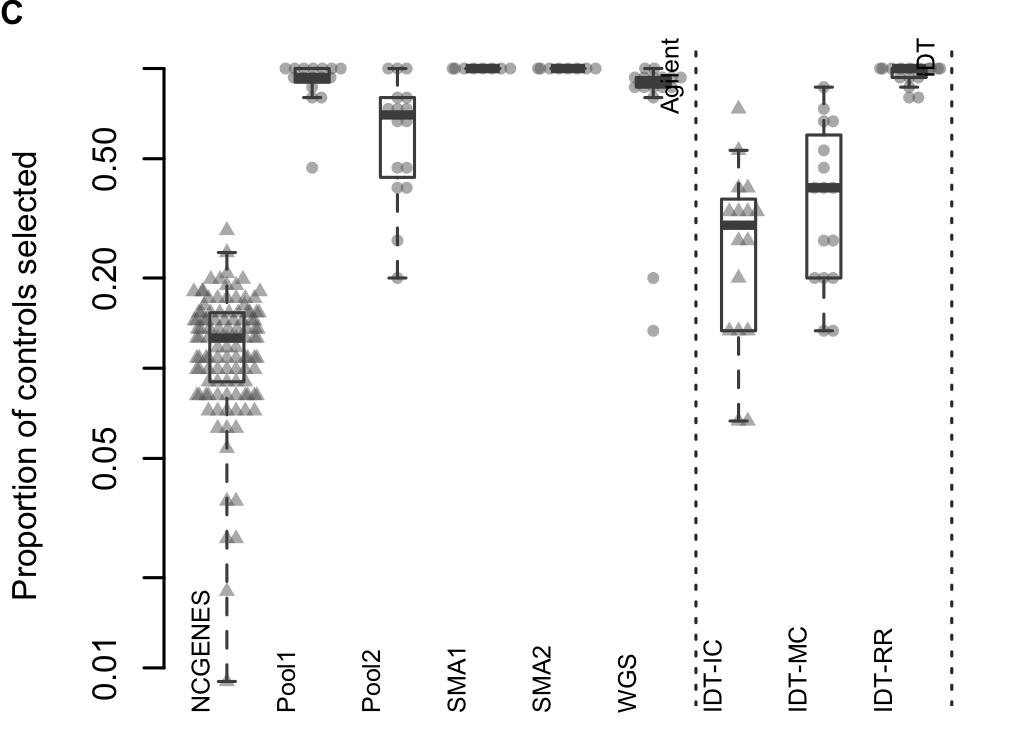
\includegraphics[]{figures-edSelection-3.pdf}%
  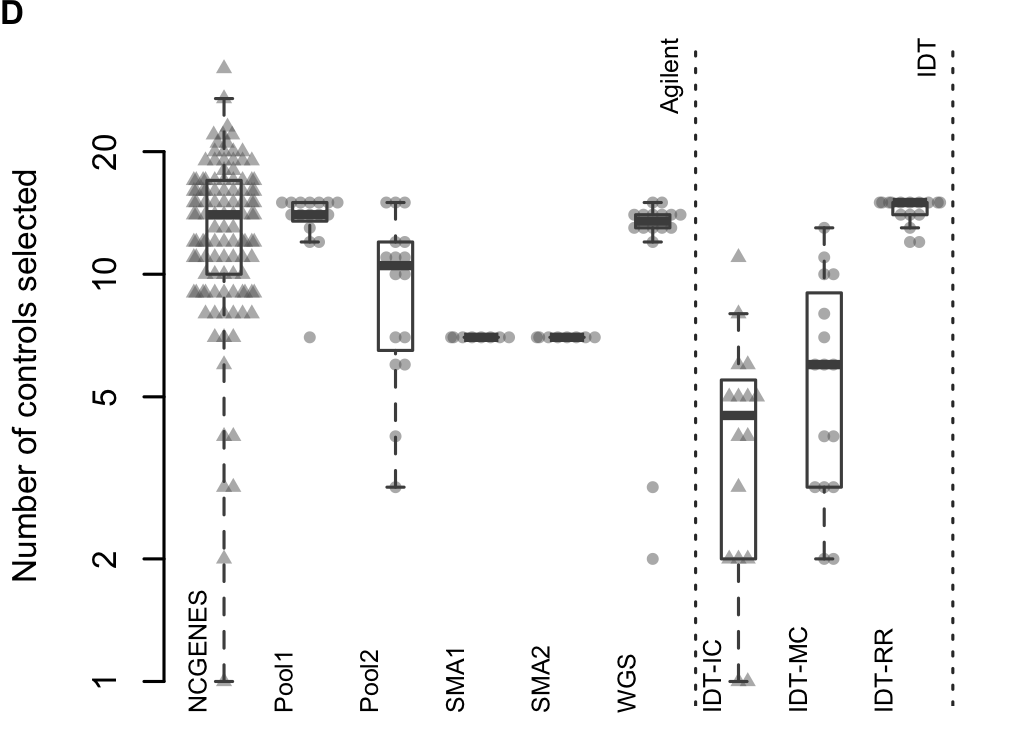
\includegraphics[]{figures-edSelection-4.pdf}
  \caption{manuscript figure}
\end{figure}

\newpage
\section{Comparing calls on simulation study}

\begin{knitrout}
\definecolor{shadecolor}{rgb}{0.969, 0.969, 0.969}\color{fgcolor}\begin{kframe}
\begin{alltt}
\hlkwd{data}\hlstd{(simRes)}
\hlstd{procSimRes} \hlkwb{<-} \hlkwd{lapply}\hlstd{(simRes,} \hlkwa{function}\hlstd{(}\hlkwc{x}\hlstd{)} \hlkwd{procRes}\hlstd{(x}\hlopt{$}\hlstd{clpRes))}

\hlstd{simResTbl} \hlkwb{<-} \hlkwd{lapply}\hlstd{(procSimRes,}
                    \hlkwa{function}\hlstd{(}\hlkwc{x}\hlstd{) x}\hlopt{$}\hlstd{mnDat[ ,} \hlkwd{.}\hlstd{(mcc, tpr, fdr),} \hlkwc{keyby} \hlstd{= dep])}
\hlstd{simResTbl} \hlkwb{<-} \hlkwd{Reduce}\hlstd{(merge, simResTbl)}
\hlkwd{setnames}\hlstd{(simResTbl,}
         \hlkwd{c}\hlstd{(}\hlstr{"dep"}\hlstd{,}
           \hlstr{"mcMCC"}\hlstd{,} \hlstr{"mcTPR"}\hlstd{,} \hlstr{"mcFDR"}\hlstd{,}  \hlcom{## mcCNV}
           \hlstr{"edMCC"}\hlstd{,} \hlstr{"edTPR"}\hlstd{,} \hlstr{"edFDR"}\hlstd{,}  \hlcom{## ExomeDepthDefault}
           \hlstr{"ebMCC"}\hlstd{,} \hlstr{"ebTPR"}\hlstd{,} \hlstr{"ebFDR"}\hlstd{))} \hlcom{## ExomeDepthBest}
\hlkwd{setcolorder}\hlstd{(simResTbl,}
            \hlkwd{c}\hlstd{(}\hlstr{"dep"}\hlstd{,} \hlstr{"mcMCC"}\hlstd{,} \hlstr{"edMCC"}\hlstd{,} \hlstr{"ebMCC"}\hlstd{,} \hlstr{"mcTPR"}\hlstd{,}
              \hlstr{"edTPR"}\hlstd{,} \hlstr{"ebTPR"}\hlstd{,} \hlstr{"mcFDR"}\hlstd{,} \hlstr{"edFDR"}\hlstd{,} \hlstr{"ebFDR"}\hlstd{))}
\hlstd{simResTbl} \hlkwb{<-} \hlstd{simResTbl[ ,} \hlkwd{lapply}\hlstd{(.SD, signif,} \hlnum{3}\hlstd{),} \hlkwc{by} \hlstd{= dep]}
\hlstd{simResTbl}
\end{alltt}
\begin{verbatim}
##     dep mcMCC edMCC ebMCC mcTPR edTPR ebTPR   mcFDR   edFDR   ebFDR
##  1:   5 0.713 0.401 0.519 0.522 0.192 0.298 0.02230 0.15900 0.09260
##  2:  10 0.694 0.628 0.708 0.503 0.431 0.549 0.04250 0.08450 0.08590
##  3:  15 0.781 0.742 0.801 0.627 0.581 0.690 0.02600 0.05270 0.06940
##  4:  20 0.840 0.811 0.857 0.719 0.682 0.777 0.01810 0.03420 0.05360
##  5:  25 0.879 0.856 0.893 0.783 0.752 0.832 0.01310 0.02460 0.04090
##  6:  30 0.907 0.889 0.918 0.831 0.804 0.872 0.00967 0.01750 0.03210
##  7:  35 0.926 0.909 0.935 0.864 0.839 0.897 0.00807 0.01370 0.02600
##  8:  40 0.941 0.927 0.948 0.891 0.869 0.917 0.00638 0.01060 0.02080
##  9:  45 0.952 0.940 0.957 0.911 0.892 0.932 0.00527 0.00846 0.01680
## 10:  50 0.961 0.950 0.965 0.927 0.910 0.944 0.00437 0.00701 0.01370
## 11:  55 0.966 0.957 0.969 0.937 0.921 0.951 0.00377 0.00569 0.01180
## 12:  60 0.972 0.963 0.974 0.947 0.933 0.959 0.00318 0.00517 0.00986
## 13:  65 0.976 0.969 0.978 0.955 0.943 0.964 0.00290 0.00433 0.00837
## 14:  70 0.978 0.972 0.980 0.960 0.949 0.968 0.00252 0.00381 0.00735
## 15:  75 0.981 0.976 0.983 0.965 0.955 0.972 0.00212 0.00321 0.00625
## 16:  80 0.983 0.978 0.985 0.969 0.960 0.975 0.00200 0.00294 0.00560
## 17:  85 0.985 0.980 0.986 0.972 0.963 0.977 0.00181 0.00263 0.00491
## 18:  90 0.987 0.982 0.987 0.975 0.967 0.979 0.00169 0.00243 0.00451
## 19:  95 0.988 0.984 0.988 0.978 0.970 0.981 0.00156 0.00223 0.00393
## 20: 100 0.989 0.985 0.989 0.980 0.973 0.982 0.00150 0.00195 0.00359
\end{verbatim}
\end{kframe}
\end{knitrout}


\begin{knitrout}
\definecolor{shadecolor}{rgb}{0.969, 0.969, 0.969}\color{fgcolor}\begin{kframe}
\begin{alltt}
\hlkwd{pltStatCompare}\hlstd{(}\hlkwc{xRes} \hlstd{= procSimRes}\hlopt{$}\hlstd{ExomeDepthDefault,} \hlkwc{yRes} \hlstd{= procSimRes}\hlopt{$}\hlstd{mcCNV,}
               \hlkwc{stat} \hlstd{=} \hlstr{"mcc"}\hlstd{,} \hlkwc{xlab} \hlstd{=} \hlstr{"ExomeDepth (default)"}\hlstd{,} \hlkwc{ylab} \hlstd{=} \hlstr{"mcCNV"}\hlstd{)}
\hlkwd{addfiglab}\hlstd{(}\hlstr{"A"}\hlstd{)}
\hlkwd{pltStatCompare}\hlstd{(}\hlkwc{xRes} \hlstd{= procSimRes}\hlopt{$}\hlstd{ExomeDepthDefault,} \hlkwc{yRes} \hlstd{= procSimRes}\hlopt{$}\hlstd{mcCNV,}
               \hlkwc{stat} \hlstd{=} \hlstr{"tpr"}\hlstd{,} \hlkwc{xlab} \hlstd{=} \hlstr{"ExomeDepth (default)"}\hlstd{,} \hlkwc{ylab} \hlstd{=} \hlstr{"mcCNV"}\hlstd{)}
\hlkwd{addfiglab}\hlstd{(}\hlstr{"B"}\hlstd{)}
\hlkwd{pltStatCompare}\hlstd{(}\hlkwc{xRes} \hlstd{= procSimRes}\hlopt{$}\hlstd{ExomeDepthDefault,} \hlkwc{yRes} \hlstd{= procSimRes}\hlopt{$}\hlstd{mcCNV,}
               \hlkwc{stat} \hlstd{=} \hlstr{"fdr"}\hlstd{,} \hlkwc{xlab} \hlstd{=} \hlstr{"ExomeDepth (default)"}\hlstd{,} \hlkwc{ylab} \hlstd{=} \hlstr{"mcCNV"}\hlstd{)}
\hlkwd{addfiglab}\hlstd{(}\hlstr{"C"}\hlstd{)}
\hlkwd{pltStatCompare}\hlstd{(}\hlkwc{xRes} \hlstd{= procSimRes}\hlopt{$}\hlstd{ExomeDepthBest,} \hlkwc{yRes} \hlstd{= procSimRes}\hlopt{$}\hlstd{mcCNV,}
               \hlkwc{stat} \hlstd{=} \hlstr{"mcc"}\hlstd{,} \hlkwc{xlab} \hlstd{=} \hlstr{"ExomeDepth (correct)"}\hlstd{,} \hlkwc{ylab} \hlstd{=} \hlstr{"mcCNV"}\hlstd{)}
\hlkwd{addfiglab}\hlstd{(}\hlstr{"D"}\hlstd{)}
\hlkwd{pltStatCompare}\hlstd{(}\hlkwc{xRes} \hlstd{= procSimRes}\hlopt{$}\hlstd{ExomeDepthBest,} \hlkwc{yRes} \hlstd{= procSimRes}\hlopt{$}\hlstd{mcCNV,}
               \hlkwc{stat} \hlstd{=} \hlstr{"tpr"}\hlstd{,} \hlkwc{xlab} \hlstd{=} \hlstr{"ExomeDepth (correct)"}\hlstd{,} \hlkwc{ylab} \hlstd{=} \hlstr{"mcCNV"}\hlstd{)}
\hlkwd{addfiglab}\hlstd{(}\hlstr{"E"}\hlstd{)}
\hlkwd{pltStatCompare}\hlstd{(}\hlkwc{xRes} \hlstd{= procSimRes}\hlopt{$}\hlstd{ExomeDepthBest,} \hlkwc{yRes} \hlstd{= procSimRes}\hlopt{$}\hlstd{mcCNV,}
               \hlkwc{stat} \hlstd{=} \hlstr{"fdr"}\hlstd{,} \hlkwc{xlab} \hlstd{=} \hlstr{"ExomeDepth (correct)"}\hlstd{,} \hlkwc{ylab} \hlstd{=} \hlstr{"mcCNV"}\hlstd{)}
\hlkwd{addfiglab}\hlstd{(}\hlstr{"F"}\hlstd{)}
\end{alltt}
\end{kframe}
\end{knitrout}

\begin{figure}[H]
  \centering
  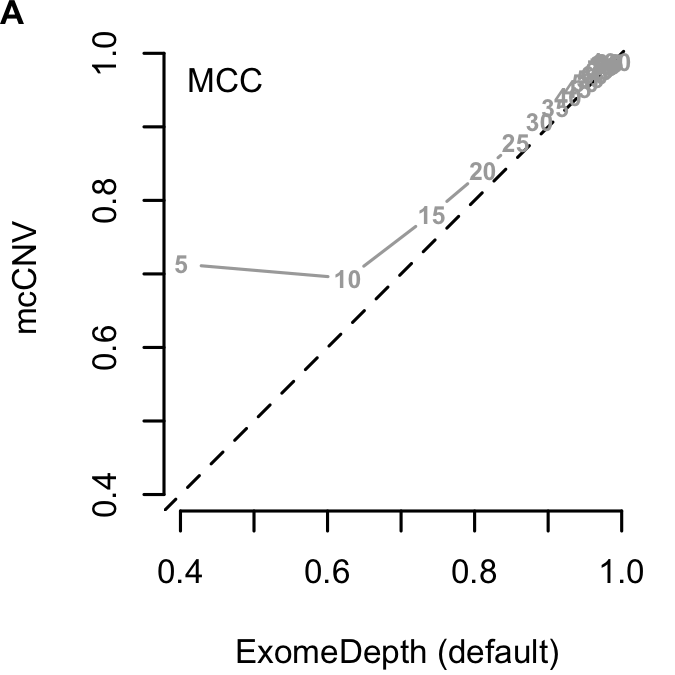
\includegraphics[]{figures-simPlts-1.pdf}%
  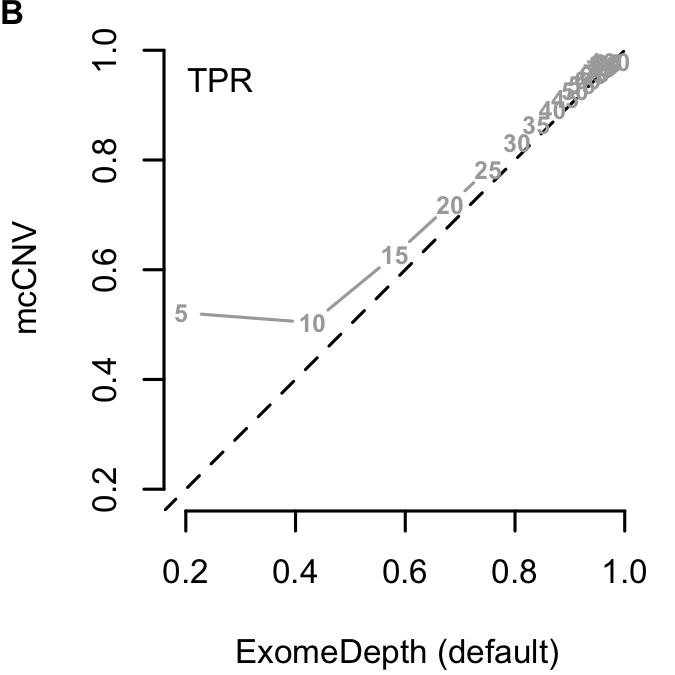
\includegraphics[]{figures-simPlts-2.pdf}%
  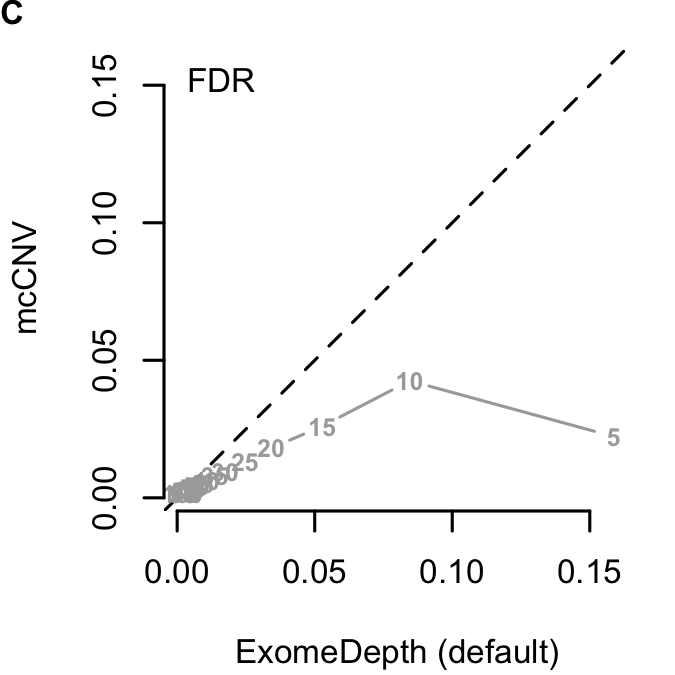
\includegraphics[]{figures-simPlts-3.pdf}
  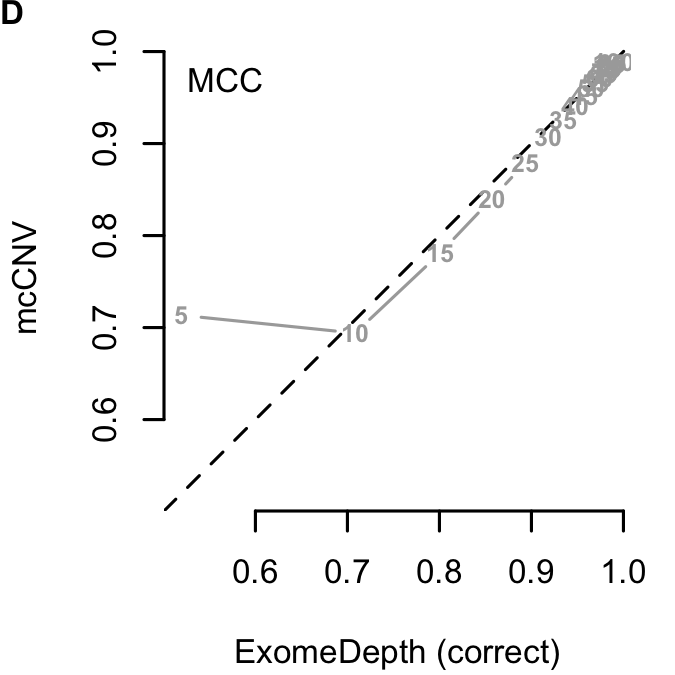
\includegraphics[]{figures-simPlts-4.pdf}%
  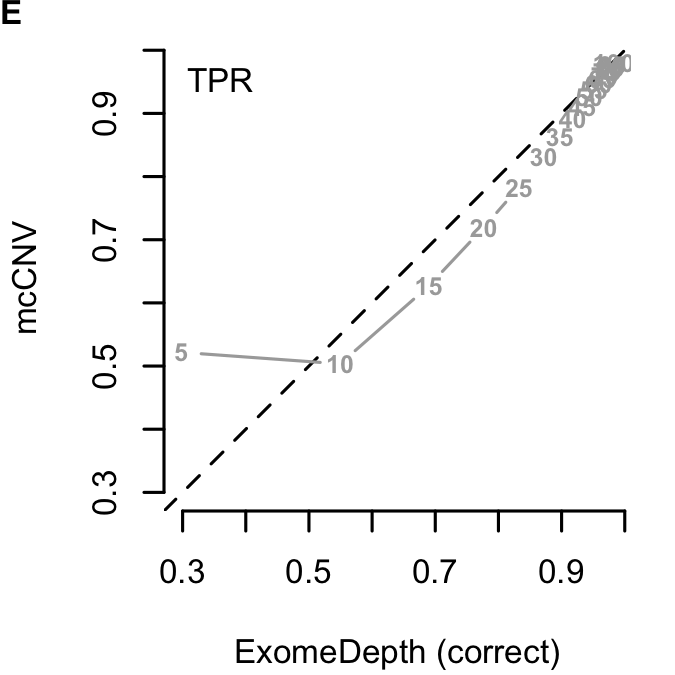
\includegraphics[]{figures-simPlts-5.pdf}%
  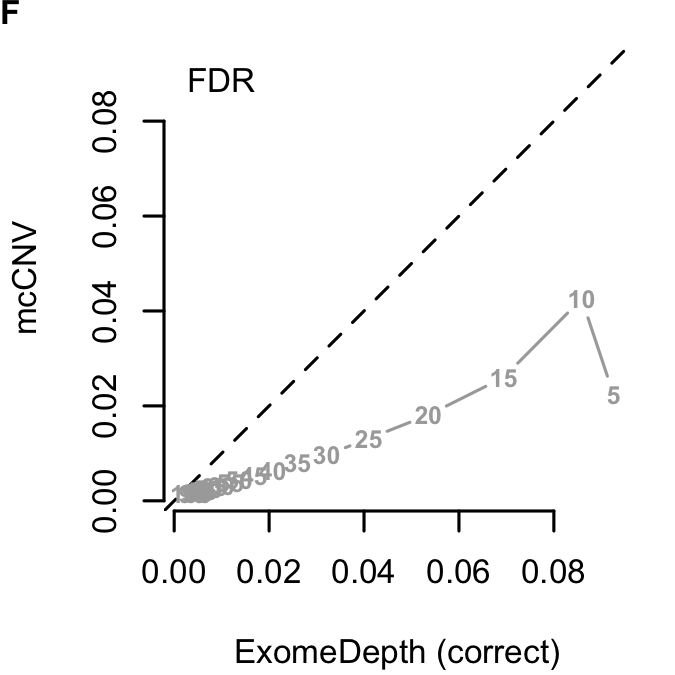
\includegraphics[]{figures-simPlts-6.pdf}
  \caption{}
\end{figure}

\newpage
\section{Comparing calls on WGS pool}

\begin{knitrout}
\definecolor{shadecolor}{rgb}{0.969, 0.969, 0.969}\color{fgcolor}\begin{kframe}
\begin{alltt}
\hlkwd{data}\hlstd{(wgsPoolCalls)}
\hlstd{mergeAll} \hlkwb{<-} \hlkwa{function}\hlstd{(}\hlkwc{x}\hlstd{,} \hlkwc{y}\hlstd{)} \hlkwd{merge}\hlstd{(x, y,} \hlkwc{all} \hlstd{=} \hlnum{TRUE}\hlstd{)}
\hlstd{wgs} \hlkwb{<-} \hlkwd{Reduce}\hlstd{(mergeAll, wgsPoolCalls)}
\hlkwd{data}\hlstd{(intAgl)}
\hlstd{xpandInt} \hlkwb{<-} \hlkwa{function}\hlstd{(}\hlkwc{int}\hlstd{,} \hlkwc{sbjVec}\hlstd{) \{}
  \hlstd{lst} \hlkwb{<-} \hlkwd{vector}\hlstd{(}\hlkwc{mode} \hlstd{=} \hlstr{"list"}\hlstd{,} \hlkwc{length} \hlstd{=} \hlkwd{length}\hlstd{(sbjVec))}
  \hlkwd{names}\hlstd{(lst)} \hlkwb{<-} \hlstd{sbjVec}
  \hlkwa{for} \hlstd{(s} \hlkwa{in} \hlstd{sbjVec) \{}
    \hlstd{lst[[s]]} \hlkwb{<-} \hlkwd{copy}\hlstd{(int)}
    \hlstd{lst[[s]][ , subject} \hlkwb{:=} \hlstd{s]}
  \hlstd{\}}
  \hlkwd{rbindlist}\hlstd{(lst)}
\hlstd{\}}
\hlstd{wgsAgl} \hlkwb{<-} \hlkwd{xpandInt}\hlstd{(intAgl, wgs[ ,} \hlkwd{unique}\hlstd{(subject)])}
\hlkwd{setkeyv}\hlstd{(wgsAgl,} \hlkwd{key}\hlstd{(wgs))}
\hlstd{wgs} \hlkwb{<-} \hlstd{wgs[wgsAgl]}
\hlkwd{rm}\hlstd{(wgsAgl)}
\hlstd{wgs} \hlkwb{<-} \hlstd{wgs[}\hlopt{!}\hlstd{(rlcr),}
           \hlkwd{.}\hlstd{(}\hlkwc{mcDup} \hlstd{=} \hlopt{!}\hlkwd{is.na}\hlstd{(passFilter)} \hlopt{&} \hlstd{CN} \hlopt{>} \hlnum{1}\hlstd{,}
             \hlkwc{edDup} \hlstd{=} \hlopt{!}\hlkwd{is.na}\hlstd{(type)} \hlopt{&} \hlstd{type} \hlopt{==} \hlstr{"duplication"}\hlstd{,}
             \hlkwc{wgDup} \hlstd{=} \hlopt{!}\hlkwd{is.na}\hlstd{(erds)} \hlopt{& !}\hlkwd{is.na}\hlstd{(cnvpytor)} \hlopt{&} \hlstd{erds} \hlopt{==} \hlstr{"dup"}\hlstd{,}
             \hlkwc{mcDel} \hlstd{=} \hlopt{!}\hlkwd{is.na}\hlstd{(passFilter)} \hlopt{&} \hlstd{CN} \hlopt{<} \hlnum{1}\hlstd{,}
             \hlkwc{edDel} \hlstd{=} \hlopt{!}\hlkwd{is.na}\hlstd{(type)} \hlopt{&} \hlstd{type} \hlopt{==} \hlstr{"deletion"}\hlstd{,}
             \hlkwc{wgDel} \hlstd{=} \hlopt{!}\hlkwd{is.na}\hlstd{(erds)} \hlopt{& !}\hlkwd{is.na}\hlstd{(cnvpytor)} \hlopt{&} \hlstd{erds} \hlopt{==} \hlstr{"del"}\hlstd{),}
           \hlkwc{by} \hlstd{=} \hlkwd{.}\hlstd{(subject, seqnames, start, end)]}
\hlstd{wgs[ , mc} \hlkwb{:=} \hlstd{mcDup} \hlopt{|} \hlstd{mcDel]}
\hlstd{wgs[ , ed} \hlkwb{:=} \hlstd{edDup} \hlopt{|} \hlstd{edDel]}
\hlstd{wgs[ , wg} \hlkwb{:=} \hlstd{wgDup} \hlopt{|} \hlstd{wgDel]}
\hlkwd{setcolorder}\hlstd{(wgs,} \hlkwd{c}\hlstd{(}\hlkwd{key}\hlstd{(wgs),} \hlstr{'mc'}\hlstd{,} \hlstr{'ed'}\hlstd{,} \hlstr{'wg'}\hlstd{))}
\hlstd{wgsCallBySbj} \hlkwb{<-} \hlstd{wgs[ ,} \hlkwd{lapply}\hlstd{(.SD, sum),} \hlkwc{.SDcols} \hlstd{= is.logical,} \hlkwc{by} \hlstd{= subject]}
\hlstd{wgsCallBySbj}
\end{alltt}
\begin{verbatim}
##       subject   mc   ed  wg mcDup edDup wgDup mcDel edDel wgDel
##  1: NCG_00012   90  106 143    61    73   121    29    33    22
##  2: NCG_00237   82  101 165    50    64   129    32    37    36
##  3: NCG_00525   68   74 151    30    33   110    38    41    41
##  4: NCG_00593   45   58 142    22    28    81    23    30    61
##  5: NCG_00676   66   78 112    38    46    92    28    32    20
##  6: NCG_00790 5156 2204 121    19    37    92  5137  2167    29
##  7: NCG_00819   68   76 134    30    41   100    38    35    34
##  8: NCG_00840   78   92 157    44    52   115    34    40    42
##  9: NCG_00851 1151  859 141    28    51   102  1123   808    39
## 10: NCG_00857   59   75 119    10    15    81    49    60    38
## 11: NCG_00976   46   58 114    25    37    93    21    21    21
## 12: NCG_01023   59   95 143    32    60   113    27    35    30
## 13: NCG_01043   73   94 128    40    64   105    33    30    23
## 14: NCG_01076   36   57 105     7    22    78    29    35    27
## 15: NCG_01077  135  157 230   103   121   184    32    36    46
## 16: NCG_01117   95  101 154    72    78   129    23    23    25
\end{verbatim}
\end{kframe}
\end{knitrout}

\begin{knitrout}
\definecolor{shadecolor}{rgb}{0.969, 0.969, 0.969}\color{fgcolor}\begin{kframe}
\begin{alltt}
\hlstd{wgs[ ,}
    \hlkwd{c}\hlstd{(}\hlstr{"mcRunID"}\hlstd{,} \hlstr{"edRunID"}\hlstd{,} \hlstr{"wgRunID"}\hlstd{)} \hlkwb{:=}
      \hlkwd{.}\hlstd{(}\hlkwd{paste}\hlstd{(subject, seqnames,} \hlkwd{rleid}\hlstd{(mc),} \hlkwc{sep} \hlstd{=} \hlstr{":"}\hlstd{),}
        \hlkwd{paste}\hlstd{(subject, seqnames,} \hlkwd{rleid}\hlstd{(ed),} \hlkwc{sep} \hlstd{=} \hlstr{":"}\hlstd{),}
        \hlkwd{paste}\hlstd{(subject, seqnames,} \hlkwd{rleid}\hlstd{(wg),} \hlkwc{sep} \hlstd{=} \hlstr{":"}\hlstd{)),}
    \hlkwc{by} \hlstd{=} \hlkwd{.}\hlstd{(subject, seqnames)]}
\hlstd{wgs[}\hlopt{!}\hlstd{(mc), mcRunID} \hlkwb{:=} \hlnum{NA_character_}\hlstd{]}
\hlstd{wgs[}\hlopt{!}\hlstd{(ed), edRunID} \hlkwb{:=} \hlnum{NA_character_}\hlstd{]}
\hlstd{wgs[}\hlopt{!}\hlstd{(wg), wgRunID} \hlkwb{:=} \hlnum{NA_character_}\hlstd{]}
\hlstd{wgs[(mc), mcVarLen} \hlkwb{:=} \hlstd{.N,} \hlkwc{by} \hlstd{=} \hlkwd{.}\hlstd{(mcRunID)]}
\hlstd{wgs[(ed), edVarLen} \hlkwb{:=} \hlstd{.N,} \hlkwc{by} \hlstd{=} \hlkwd{.}\hlstd{(edRunID)]}
\hlstd{wgs[(wg), wgVarLen} \hlkwb{:=} \hlstd{.N,} \hlkwc{by} \hlstd{=} \hlkwd{.}\hlstd{(wgRunID)]}

\hlcom{## Count number of variants by variant length for each algorithm}
\hlstd{mergeAll} \hlkwb{<-} \hlkwa{function}\hlstd{(}\hlkwc{x}\hlstd{,} \hlkwc{y}\hlstd{)} \hlkwd{merge}\hlstd{(x, y,} \hlkwc{all} \hlstd{=} \hlnum{TRUE}\hlstd{)}
\hlstd{wgs[}\hlopt{!}\hlstd{subject} \hlopt \hlkwd{c}\hlstd{(}\hlstr{"NCG_00790"}\hlstd{,} \hlstr{"NCG_00851"}\hlstd{), \{}
  \hlstd{lst} \hlkwb{<-} \hlkwd{list}\hlstd{(.SD[}\hlopt{!}\hlkwd{is.na}\hlstd{(mcVarLen),}
                  \hlkwd{.}\hlstd{(}\hlkwc{mc} \hlstd{=} \hlkwd{length}\hlstd{(}\hlkwd{unique}\hlstd{(mcRunID))),}
                  \hlkwc{by} \hlstd{=} \hlkwd{.}\hlstd{(}\hlkwc{varLen} \hlstd{=} \hlkwd{pmin}\hlstd{(mcVarLen,} \hlnum{10}\hlstd{))],}
              \hlstd{.SD[}\hlopt{!}\hlkwd{is.na}\hlstd{(edVarLen),}
                  \hlkwd{.}\hlstd{(}\hlkwc{ed} \hlstd{=} \hlkwd{length}\hlstd{(}\hlkwd{unique}\hlstd{(edRunID))),}
                  \hlkwc{by} \hlstd{=} \hlkwd{.}\hlstd{(}\hlkwc{varLen} \hlstd{=} \hlkwd{pmin}\hlstd{(edVarLen,} \hlnum{10}\hlstd{))],}
              \hlstd{.SD[}\hlopt{!}\hlkwd{is.na}\hlstd{(wgVarLen),}
                  \hlkwd{.}\hlstd{(}\hlkwc{wg} \hlstd{=} \hlkwd{length}\hlstd{(}\hlkwd{unique}\hlstd{(wgRunID))),}
                  \hlkwc{by} \hlstd{=} \hlkwd{.}\hlstd{(}\hlkwc{varLen} \hlstd{=} \hlkwd{pmin}\hlstd{(wgVarLen,} \hlnum{10}\hlstd{))])}
  \hlkwd{Reduce}\hlstd{(mergeAll, lst)}
\hlstd{\}]}
\end{alltt}
\begin{verbatim}
##     varLen  mc  ed  wg
##  1:      1 297 179 138
##  2:      2  78  78  78
##  3:      3  57  71 102
##  4:      4  14  17  36
##  5:      5  15  17  30
##  6:      6  12  20  15
##  7:      7   5   5   4
##  8:      8   4   6  25
##  9:      9   2   1  15
## 10:     10   6  13  42
\end{verbatim}
\begin{alltt}
\hlstd{calcOverlap} \hlkwb{<-} \hlkwa{function}\hlstd{(}\hlkwc{vl}\hlstd{,} \hlkwc{exclude} \hlstd{=} \hlkwd{c}\hlstd{(}\hlstr{"NCG_00790"}\hlstd{,} \hlstr{"NCG_00851"}\hlstd{)) \{}
  \hlstd{mc} \hlkwb{<-} \hlstd{wgs[}\hlopt{!}\hlstd{subject} \hlopt \hlstd{exclude][}\hlkwd{pmin}\hlstd{(mcVarLen,} \hlnum{10}\hlstd{)} \hlopt{==} \hlstd{vl]}
  \hlstd{mc} \hlkwb{<-} \hlstd{mc[ ,} \hlkwd{.}\hlstd{(}\hlkwc{wg} \hlstd{=} \hlkwd{any}\hlstd{(wg),} \hlkwc{ed} \hlstd{=} \hlkwd{any}\hlstd{(ed)),} \hlkwc{by} \hlstd{=} \hlkwd{.}\hlstd{(mcRunID)]}
  \hlstd{mc} \hlkwb{<-} \hlstd{mc[ ,} \hlkwd{.}\hlstd{(}\hlkwc{vl} \hlstd{= vl,} \hlkwc{prd} \hlstd{=} \hlstr{"mc"}\hlstd{,} \hlkwc{wg} \hlstd{=} \hlkwd{sum}\hlstd{(wg)}\hlopt{/}\hlstd{.N,} \hlkwc{ed} \hlstd{=} \hlkwd{sum}\hlstd{(ed)}\hlopt{/}\hlstd{.N)]}
  \hlstd{mc} \hlkwb{<-} \hlkwd{melt}\hlstd{(mc,} \hlkwc{id.vars} \hlstd{=} \hlkwd{c}\hlstd{(}\hlstr{"vl"}\hlstd{,} \hlstr{"prd"}\hlstd{))}

  \hlstd{ed} \hlkwb{<-} \hlstd{wgs[}\hlopt{!}\hlstd{subject} \hlopt \hlstd{exclude][}\hlkwd{pmin}\hlstd{(edVarLen,} \hlnum{10}\hlstd{)} \hlopt{==} \hlstd{vl]}
  \hlstd{ed} \hlkwb{<-} \hlstd{ed[ ,} \hlkwd{.}\hlstd{(}\hlkwc{wg} \hlstd{=} \hlkwd{any}\hlstd{(wg),} \hlkwc{mc} \hlstd{=} \hlkwd{any}\hlstd{(mc)),} \hlkwc{by} \hlstd{=} \hlkwd{.}\hlstd{(edRunID)]}
  \hlstd{ed} \hlkwb{<-} \hlstd{ed[ ,} \hlkwd{.}\hlstd{(}\hlkwc{vl} \hlstd{= vl,} \hlkwc{prd} \hlstd{=} \hlstr{"ed"}\hlstd{,} \hlkwc{wg} \hlstd{=} \hlkwd{sum}\hlstd{(wg)}\hlopt{/}\hlstd{.N,} \hlkwc{mc} \hlstd{=} \hlkwd{sum}\hlstd{(mc)}\hlopt{/}\hlstd{.N)]}
  \hlstd{ed} \hlkwb{<-} \hlkwd{melt}\hlstd{(ed,} \hlkwc{id.vars} \hlstd{=} \hlkwd{c}\hlstd{(}\hlstr{"vl"}\hlstd{,} \hlstr{"prd"}\hlstd{))}

  \hlstd{wg} \hlkwb{<-} \hlstd{wgs[}\hlopt{!}\hlstd{subject} \hlopt \hlstd{exclude][}\hlkwd{pmin}\hlstd{(wgVarLen,} \hlnum{10}\hlstd{)} \hlopt{==} \hlstd{vl]}
  \hlstd{wg} \hlkwb{<-} \hlstd{wg[ ,} \hlkwd{.}\hlstd{(}\hlkwc{mc} \hlstd{=} \hlkwd{any}\hlstd{(mc),} \hlkwc{ed} \hlstd{=} \hlkwd{any}\hlstd{(ed)),} \hlkwc{by} \hlstd{=} \hlkwd{.}\hlstd{(wgRunID)]}
  \hlstd{wg} \hlkwb{<-} \hlstd{wg[ ,} \hlkwd{.}\hlstd{(}\hlkwc{vl} \hlstd{= vl,} \hlkwc{prd} \hlstd{=} \hlstr{"wg"}\hlstd{,} \hlkwc{mc} \hlstd{=} \hlkwd{sum}\hlstd{(mc)}\hlopt{/}\hlstd{.N,} \hlkwc{ed} \hlstd{=} \hlkwd{sum}\hlstd{(ed)}\hlopt{/}\hlstd{.N)]}
  \hlstd{wg} \hlkwb{<-} \hlkwd{melt}\hlstd{(wg,} \hlkwc{id.vars} \hlstd{=} \hlkwd{c}\hlstd{(}\hlstr{"vl"}\hlstd{,} \hlstr{"prd"}\hlstd{))}

  \hlstd{res} \hlkwb{<-} \hlkwd{rbindlist}\hlstd{(}\hlkwd{list}\hlstd{(mc, ed, wg))}
  \hlstd{res[ ,} \hlkwd{.}\hlstd{(vl, prd,} \hlkwc{tst} \hlstd{=} \hlkwd{as.character}\hlstd{(variable),} \hlkwc{pct} \hlstd{=} \hlkwd{round}\hlstd{(value,} \hlnum{3}\hlstd{))][]}
\hlstd{\}}
\hlcom{## Percentage of calls predicted (prd) found in the other algorithms (tst)}
\hlcom{## by variant length (vl)}
\hlstd{callByVarLen} \hlkwb{<-} \hlkwd{rbindlist}\hlstd{(}\hlkwd{lapply}\hlstd{(}\hlnum{1}\hlopt{:}\hlnum{10}\hlstd{, calcOverlap))[}\hlkwd{order}\hlstd{(vl, prd, tst)]}
\hlkwd{cbind}\hlstd{(callByVarLen[}\hlnum{1}\hlopt{:}\hlnum{30}\hlstd{], callByVarLen[}\hlnum{31}\hlopt{:}\hlnum{60}\hlstd{])}
\end{alltt}
\begin{verbatim}
##     vl prd tst   pct vl prd tst   pct
##  1:  1  ed  mc 0.732  6  ed  mc 1.000
##  2:  1  ed  wg 0.341  6  ed  wg 0.650
##  3:  1  mc  ed 0.700  6  mc  ed 1.000
##  4:  1  mc  wg 0.374  6  mc  wg 0.917
##  5:  1  wg  ed 0.391  6  wg  ed 0.800
##  6:  1  wg  mc 0.478  6  wg  mc 1.000
##  7:  2  ed  mc 0.808  7  ed  mc 0.800
##  8:  2  ed  wg 0.577  7  ed  wg 0.600
##  9:  2  mc  ed 0.885  7  mc  ed 1.000
## 10:  2  mc  wg 0.615  7  mc  wg 1.000
## 11:  2  wg  ed 0.654  7  wg  ed 0.250
## 12:  2  wg  mc 0.538  7  wg  mc 0.250
## 13:  3  ed  mc 0.831  8  ed  mc 1.000
## 14:  3  ed  wg 0.662  8  ed  wg 0.500
## 15:  3  mc  ed 0.912  8  mc  ed 1.000
## 16:  3  mc  wg 0.737  8  mc  wg 1.000
## 17:  3  wg  ed 0.392  8  wg  ed 0.240
## 18:  3  wg  mc 0.451  8  wg  mc 0.160
## 19:  4  ed  mc 1.000  9  ed  mc 1.000
## 20:  4  ed  wg 0.471  9  ed  wg 1.000
## 21:  4  mc  ed 1.000  9  mc  ed 1.000
## 22:  4  mc  wg 1.000  9  mc  wg 1.000
## 23:  4  wg  ed 0.278  9  wg  ed 0.067
## 24:  4  wg  mc 0.444  9  wg  mc 0.067
## 25:  5  ed  mc 0.882 10  ed  mc 1.000
## 26:  5  ed  wg 0.353 10  ed  wg 0.846
## 27:  5  mc  ed 1.000 10  mc  ed 1.000
## 28:  5  mc  wg 1.000 10  mc  wg 1.000
## 29:  5  wg  ed 0.433 10  wg  ed 0.310
## 30:  5  wg  mc 0.433 10  wg  mc 0.310
##     vl prd tst   pct vl prd tst   pct
\end{verbatim}
\end{kframe}
\end{knitrout}

\begin{knitrout}
\definecolor{shadecolor}{rgb}{0.969, 0.969, 0.969}\color{fgcolor}\begin{kframe}
\begin{alltt}
\hlstd{pmLst} \hlkwb{<-} \hlkwd{list}\hlstd{()}
\hlstd{pmLst}\hlopt{$}\hlstd{mc} \hlkwb{<-} \hlkwd{with}\hlstd{(wgs,} \hlkwd{evalPred}\hlstd{(mc, wg))}
\hlstd{pmLst}\hlopt{$}\hlstd{ed} \hlkwb{<-} \hlkwd{with}\hlstd{(wgs,} \hlkwd{evalPred}\hlstd{(ed, wg))}
\hlstd{pmLst}\hlopt{$}\hlstd{mcSub} \hlkwb{<-} \hlkwd{with}\hlstd{(wgs[}\hlopt{!}\hlkwd{grepl}\hlstd{(}\hlstr{"790|851"}\hlstd{, subject)],} \hlkwd{evalPred}\hlstd{(mc, wg))}
\hlstd{pmLst}\hlopt{$}\hlstd{edSub} \hlkwb{<-} \hlkwd{with}\hlstd{(wgs[}\hlopt{!}\hlkwd{grepl}\hlstd{(}\hlstr{"790|851"}\hlstd{, subject)],} \hlkwd{evalPred}\hlstd{(ed, wg))}
\hlstd{pmLst}\hlopt{$}\hlstd{mcDup} \hlkwb{<-} \hlkwd{with}\hlstd{(wgs,} \hlkwd{evalPred}\hlstd{(mcDup, wgDup))}
\hlstd{pmLst}\hlopt{$}\hlstd{edDup} \hlkwb{<-} \hlkwd{with}\hlstd{(wgs,} \hlkwd{evalPred}\hlstd{(edDup, wgDup))}
\hlstd{pmLst}\hlopt{$}\hlstd{mcSubDup} \hlkwb{<-} \hlkwd{with}\hlstd{(wgs[}\hlopt{!}\hlkwd{grepl}\hlstd{(}\hlstr{"790|851"}\hlstd{, subject)],}
                       \hlkwd{evalPred}\hlstd{(mcDup, wgDup))}
\hlstd{pmLst}\hlopt{$}\hlstd{edSubDup} \hlkwb{<-} \hlkwd{with}\hlstd{(wgs[}\hlopt{!}\hlkwd{grepl}\hlstd{(}\hlstr{"790|851"}\hlstd{, subject)],}
                       \hlkwd{evalPred}\hlstd{(edDup, wgDup))}
\hlstd{pmLst}\hlopt{$}\hlstd{mcDel} \hlkwb{<-} \hlkwd{with}\hlstd{(wgs,} \hlkwd{evalPred}\hlstd{(mcDel, wgDel))}
\hlstd{pmLst}\hlopt{$}\hlstd{edDel} \hlkwb{<-} \hlkwd{with}\hlstd{(wgs,} \hlkwd{evalPred}\hlstd{(edDel, wgDel))}
\hlstd{pmLst}\hlopt{$}\hlstd{mcSubDel} \hlkwb{<-} \hlkwd{with}\hlstd{(wgs[}\hlopt{!}\hlkwd{grepl}\hlstd{(}\hlstr{"790|851"}\hlstd{, subject)],}
                       \hlkwd{evalPred}\hlstd{(mcDel, wgDel))}
\hlstd{pmLst}\hlopt{$}\hlstd{edSubDel} \hlkwb{<-} \hlkwd{with}\hlstd{(wgs[}\hlopt{!}\hlkwd{grepl}\hlstd{(}\hlstr{"790|851"}\hlstd{, subject)],}
                       \hlkwd{evalPred}\hlstd{(edDel, wgDel))}
\hlstd{predMetrics} \hlkwb{<-} \hlkwd{as.data.table}\hlstd{(}\hlkwd{do.call}\hlstd{(rbind, pmLst),} \hlkwc{keep.rownames} \hlstd{=} \hlstr{"PredSet"}\hlstd{)}
\hlstd{predMetrics}
\end{alltt}
\begin{verbatim}
##      PredSet   MCC   TPR   FDR    PPV BalAcc
##  1:       mc 0.185 0.335 0.897 0.1030  0.666
##  2:       ed 0.263 0.363 0.809 0.1910  0.681
##  3:    mcSub 0.487 0.345 0.311 0.6890  0.672
##  4:    edSub 0.482 0.378 0.383 0.6170  0.689
##  5:    mcDup 0.396 0.236 0.334 0.6660  0.618
##  6:    edDup 0.347 0.240 0.496 0.5040  0.620
##  7: mcSubDup 0.404 0.246 0.333 0.6670  0.623
##  8: edSubDup 0.384 0.266 0.446 0.5540  0.633
##  9:    mcDel 0.180 0.639 0.949 0.0509  0.818
## 10:    edDel 0.219 0.558 0.914 0.0861  0.778
## 11: mcSubDel 0.683 0.661 0.294 0.7060  0.830
## 12: edSubDel 0.541 0.554 0.471 0.5290  0.777
\end{verbatim}
\end{kframe}
\end{knitrout}

\newpage
\begin{knitrout}
\definecolor{shadecolor}{rgb}{0.969, 0.969, 0.969}\color{fgcolor}\begin{kframe}
\begin{alltt}
\hlstd{ctsAll} \hlkwb{<-} \hlkwd{euler}\hlstd{(wgs[ ,} \hlkwd{.}\hlstd{(mc, ed, wg)])}
\hlstd{ctsSub} \hlkwb{<-} \hlkwd{euler}\hlstd{(wgs[}\hlopt{!}\hlkwd{grepl}\hlstd{(}\hlstr{"790|851"}\hlstd{, subject),} \hlkwd{.}\hlstd{(mc, ed, wg)])}
\hlstd{ctsAllDup} \hlkwb{<-} \hlkwd{euler}\hlstd{(wgs[ ,} \hlkwd{.}\hlstd{(mcDup, edDup, wgDup)])}
\hlstd{ctsSubDup} \hlkwb{<-} \hlkwd{euler}\hlstd{(wgs[}\hlopt{!}\hlkwd{grepl}\hlstd{(}\hlstr{"790|851"}\hlstd{, subject),} \hlkwd{.}\hlstd{(mcDup, edDup, wgDup)])}
\hlstd{ctsAllDel} \hlkwb{<-} \hlkwd{euler}\hlstd{(wgs[ ,} \hlkwd{.}\hlstd{(mcDel, edDel, wgDel)])}
\hlstd{ctsSubDel} \hlkwb{<-} \hlkwd{euler}\hlstd{(wgs[}\hlopt{!}\hlkwd{grepl}\hlstd{(}\hlstr{"790|851"}\hlstd{, subject),} \hlkwd{.}\hlstd{(mcDel, edDel, wgDel)])}
\hlkwd{eulerr_options}\hlstd{(}\hlkwc{fills} \hlstd{=} \hlkwd{list}\hlstd{(}\hlkwc{fill} \hlstd{=} \hlkwd{c}\hlstd{(}\hlstr{"#E9E9E9"}\hlstd{,} \hlstr{"#7F7FC4"}\hlstd{,} \hlstr{"#FFC57F"}\hlstd{)),}
               \hlkwc{quantities} \hlstd{=} \hlkwd{list}\hlstd{(}\hlkwc{cex} \hlstd{=} \hlnum{0.5}\hlstd{))}
\hlstd{gridFigLab} \hlkwb{<-} \hlkwa{function}\hlstd{(}\hlkwc{lab}\hlstd{) \{}
  \hlkwd{grid.text}\hlstd{(lab,} \hlkwc{x} \hlstd{=} \hlnum{0}\hlstd{,} \hlkwc{y} \hlstd{=} \hlnum{1}\hlstd{,} \hlkwc{hjust} \hlstd{=} \hlnum{0}\hlstd{,} \hlkwc{vjust} \hlstd{=} \hlnum{1}\hlstd{,} \hlkwc{gp} \hlstd{=} \hlkwd{gpar}\hlstd{(}\hlkwc{font} \hlstd{=} \hlnum{2}\hlstd{))}
\hlstd{\}}
\hlkwd{plot}\hlstd{(ctsSubDup,} \hlkwc{quantities} \hlstd{=} \hlnum{TRUE}\hlstd{,} \hlkwc{labels} \hlstd{=} \hlnum{FALSE}\hlstd{,} \hlkwc{main} \hlstd{=} \hlstr{""}\hlstd{)}
\hlkwd{gridFigLab}\hlstd{(}\hlstr{"A"}\hlstd{)}
\hlkwd{grid.text}\hlstd{(}\hlstr{"DUPLICATIONS"}\hlstd{,} \hlkwc{x} \hlstd{=} \hlnum{0.5}\hlstd{,} \hlkwc{y} \hlstd{=} \hlnum{0.9}\hlstd{)}
\hlkwd{plot}\hlstd{(ctsSubDel,} \hlkwc{quantities} \hlstd{=} \hlnum{TRUE}\hlstd{,} \hlkwc{labels} \hlstd{=} \hlnum{FALSE}\hlstd{,} \hlkwc{main} \hlstd{=} \hlstr{""}\hlstd{)}
\hlkwd{gridFigLab}\hlstd{(}\hlstr{"B"}\hlstd{)}
\hlkwd{grid.text}\hlstd{(}\hlstr{"DELETIONS"}\hlstd{,} \hlkwc{x} \hlstd{=} \hlnum{0.5}\hlstd{,} \hlkwc{y} \hlstd{=} \hlnum{0.9}\hlstd{)}
\hlkwd{plot}\hlstd{(ctsAllDup,} \hlkwc{quantities} \hlstd{=} \hlnum{TRUE}\hlstd{,} \hlkwc{labels} \hlstd{=} \hlnum{FALSE}\hlstd{,} \hlkwc{main} \hlstd{=} \hlstr{""}\hlstd{)}
\hlkwd{gridFigLab}\hlstd{(}\hlstr{"C"}\hlstd{)}
\hlkwd{grid.text}\hlstd{(}\hlstr{"DUPLICATIONS"}\hlstd{,} \hlkwc{x} \hlstd{=} \hlnum{0.5}\hlstd{,} \hlkwc{y} \hlstd{=} \hlnum{0.9}\hlstd{)}
\hlkwd{plot}\hlstd{(ctsAllDel,} \hlkwc{quantities} \hlstd{=} \hlnum{TRUE}\hlstd{,} \hlkwc{labels} \hlstd{=} \hlnum{FALSE}\hlstd{,} \hlkwc{main} \hlstd{=} \hlstr{""}\hlstd{)}
\hlkwd{gridFigLab}\hlstd{(}\hlstr{"D"}\hlstd{)}
\hlkwd{grid.text}\hlstd{(}\hlstr{"DELETIONS"}\hlstd{,} \hlkwc{x} \hlstd{=} \hlnum{0.5}\hlstd{,} \hlkwc{y} \hlstd{=} \hlnum{0.9}\hlstd{)}
\end{alltt}
\end{kframe}
\end{knitrout}

\begin{knitrout}
\definecolor{shadecolor}{rgb}{0.969, 0.969, 0.969}\color{fgcolor}\begin{kframe}
\begin{alltt}
\hlkwd{par}\hlstd{(}\hlkwc{mar} \hlstd{=} \hlkwd{rep}\hlstd{(}\hlnum{0}\hlstd{,} \hlnum{4}\hlstd{))}
\hlkwd{plot.new}\hlstd{()}
\hlkwd{legend}\hlstd{(}\hlkwc{x} \hlstd{=} \hlstr{"center"}\hlstd{,}
       \hlkwc{legend} \hlstd{=} \hlkwd{c}\hlstd{(}\hlstr{"MC"}\hlstd{,} \hlstr{"ED"}\hlstd{,} \hlstr{"WG"}\hlstd{),}
       \hlkwc{fill} \hlstd{=} \hlkwd{c}\hlstd{(}\hlstr{"#E9E9E9"}\hlstd{,} \hlstr{"#7F7FC4"}\hlstd{,} \hlstr{"#FFC57F"}\hlstd{),}
       \hlkwc{horiz} \hlstd{=} \hlnum{TRUE}\hlstd{,}
       \hlkwc{bty} \hlstd{=} \hlstr{"n"}\hlstd{)}
\end{alltt}
\end{kframe}
\end{knitrout}

\begin{figure}[H]
  \centering
  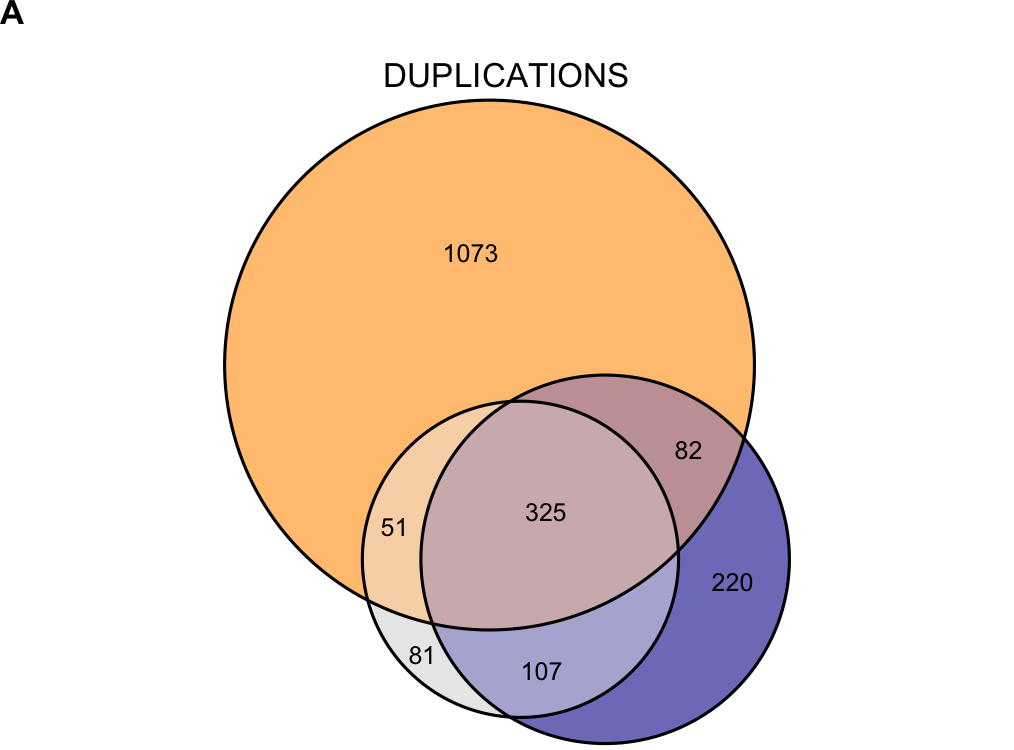
\includegraphics[]{figures-vennDiag-1.pdf}%
  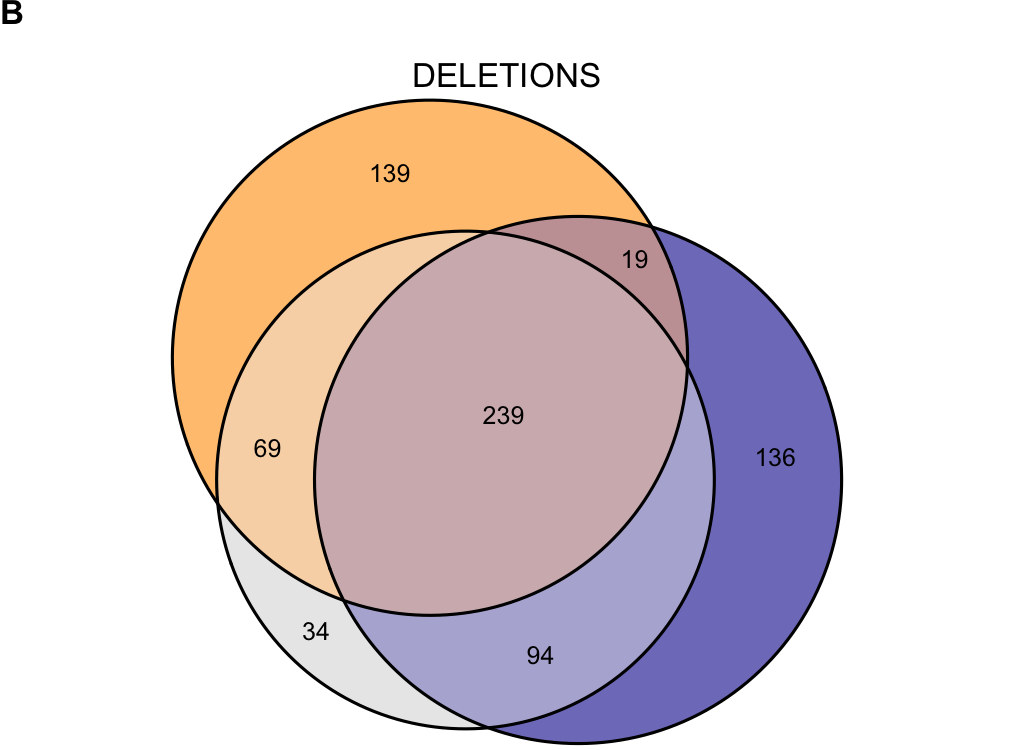
\includegraphics[]{figures-vennDiag-2.pdf}
  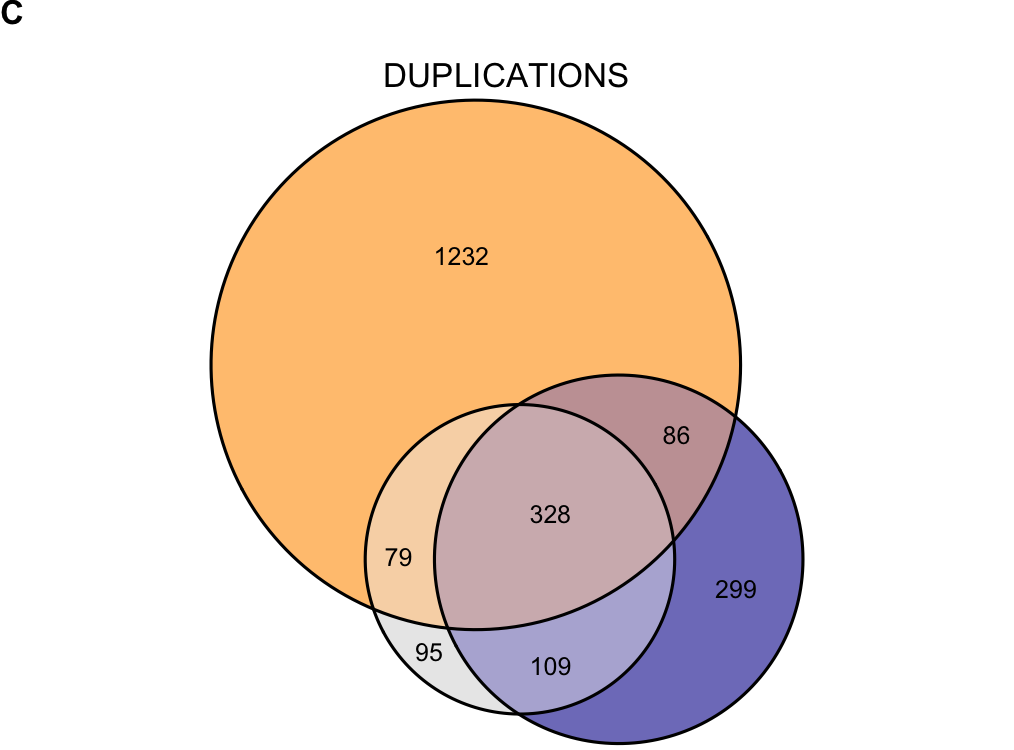
\includegraphics[]{figures-vennDiag-3.pdf}%
  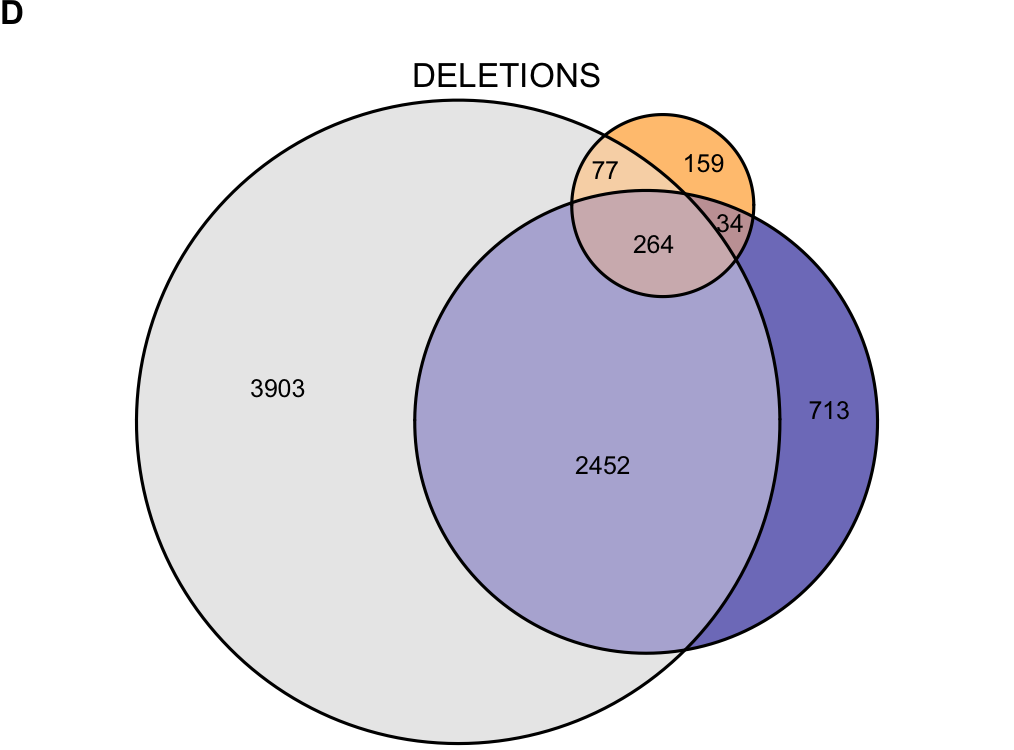
\includegraphics[]{figures-vennDiag-4.pdf}
  \includegraphics[]{figures-vennDiagLgnd-1.pdf}
  \caption{(A-B) included in manuscript; (C-D) show the concordance of duplications and deletions for the whole WGS pool. mcCNV calls in gray; ExomeDepth calls in blue; ERDS/cnvpytor calls in orange.}
\end{figure}

\section{Slurm scripts to perform simulation study}

\subsection{Create count objects}

\begin{knitrout}
\definecolor{shadecolor}{rgb}{0.969, 0.969, 0.969}\color{fgcolor}\begin{kframe}
\begin{alltt}
\hlcom{##----------------------------------------------------------------------------##}
\hlcom{## Script to create the varDepth simulated counts}
\hlcom{##----------------------------------------------------------------------------##}

\hlkwd{library}\hlstd{(mcCNV)}
\hlkwd{library}\hlstd{(rslurm)}
\hlkwd{library}\hlstd{(data.table)}
\hlkwd{library}\hlstd{(filer2020A)}

\hlcom{## Directory for storing the data}
\hlstd{wd} \hlkwb{<-} \hlkwd{getwd}\hlstd{()}

\hlkwd{data}\hlstd{(subjectMeta)}
\hlstd{pl1Int} \hlkwb{<-} \hlkwd{subsetCounts}\hlstd{(subjectMeta[pool} \hlopt{==} \hlstr{"Pool1"}\hlstd{, subject])}
\hlstd{pl1Int} \hlkwb{<-} \hlstd{pl1Int[ ,} \hlkwd{.}\hlstd{(}\hlkwc{ttl} \hlstd{=} \hlkwd{sum}\hlstd{(molCount)),} \hlkwc{by} \hlstd{=} \hlkwd{.}\hlstd{(seqnames, start, end)]}
\hlstd{pl1Int[ , captureProb} \hlkwb{:=} \hlstd{ttl}\hlopt{/}\hlkwd{sum}\hlstd{(ttl)]}
\hlstd{pl1Int[ , ttl} \hlkwb{:=} \hlkwa{NULL}\hlstd{]}

\hlstd{deps} \hlkwb{<-} \hlkwd{as.integer}\hlstd{(}\hlkwd{seq}\hlstd{(}\hlnum{5}\hlstd{,} \hlnum{100}\hlstd{,} \hlnum{5}\hlstd{))} \hlcom{## Sequencing depths}

\hlcom{## Set up the file system}
\hlstd{odir} \hlkwb{<-} \hlkwd{file.path}\hlstd{(wd,} \hlstr{"varDepthCounts"}\hlstd{)}
\hlkwa{if} \hlstd{(}\hlkwd{dir.exists}\hlstd{(odir))} \hlkwd{unlink}\hlstd{(odir,} \hlkwc{recursive} \hlstd{=} \hlnum{TRUE}\hlstd{,} \hlkwc{force} \hlstd{=} \hlnum{TRUE}\hlstd{)}
\hlkwd{dir.create}\hlstd{(odir)}

\hlstd{pars} \hlkwb{<-} \hlkwd{data.table}\hlstd{(}\hlkwd{expand.grid}\hlstd{(}\hlkwc{dep} \hlstd{= deps,} \hlkwc{rep} \hlstd{=} \hlkwd{seq}\hlstd{(}\hlnum{200}\hlstd{)))}
\hlkwd{set.seed}\hlstd{(}\hlnum{1234}\hlstd{)}
\hlstd{pars[ , seed} \hlkwb{:=} \hlkwd{sample}\hlstd{(}\hlnum{1e6}\hlstd{, .N)]}
\hlstd{pars[ , odir} \hlkwb{:=} \hlstd{odir]}

\hlstd{simPool} \hlkwb{<-} \hlkwa{function}\hlstd{(}\hlkwc{dep}\hlstd{,} \hlkwc{rep}\hlstd{,} \hlkwc{seed}\hlstd{,} \hlkwc{odir}\hlstd{) \{}
  \hlstd{wndw} \hlkwb{<-} \hlkwd{as.integer}\hlstd{(}\hlkwd{c}\hlstd{(dep} \hlopt{-} \hlnum{0.3}\hlopt{*}\hlstd{dep, dep} \hlopt{+} \hlnum{0.3}\hlopt{*}\hlstd{dep)}\hlopt{*}\hlnum{1e6}\hlstd{)}
  \hlstd{cnt} \hlkwb{<-} \hlkwd{try}\hlstd{(}\hlkwd{cnvSimPool}\hlstd{(}\hlkwc{nSubjects} \hlstd{=} \hlnum{16L}\hlstd{,}
                        \hlkwc{countRange} \hlstd{= wndw,}
                        \hlkwc{interval} \hlstd{= pl1Int,}
                        \hlkwc{seed} \hlstd{= seed,}
                        \hlkwc{variantWidth} \hlstd{=} \hlnum{1L}\hlstd{))}
  \hlstd{fname} \hlkwb{<-} \hlkwd{sprintf}\hlstd{(}\hlstr{"varDepth_d%0.3d_r%0.4d.counts"}\hlstd{, dep, rep)}
  \hlkwd{saveRDS}\hlstd{(cnt,} \hlkwc{file} \hlstd{=} \hlkwd{file.path}\hlstd{(odir, fname))}
  \hlopt{!}\hlkwd{is}\hlstd{(cnt,} \hlstr{'try-error'}\hlstd{)}
\hlstd{\}}

\hlkwd{slurm_apply}\hlstd{(}\hlkwc{f} \hlstd{= simPool,}
            \hlkwc{add_objects} \hlstd{=} \hlstr{"pl1Int"}\hlstd{,}
            \hlkwc{params} \hlstd{= pars,}
            \hlkwc{nodes} \hlstd{=} \hlkwd{nrow}\hlstd{(pars),}
            \hlkwc{cpus_per_node} \hlstd{=} \hlnum{1}\hlstd{,}
            \hlkwc{jobname} \hlstd{=} \hlstr{"varDepthCounts"}\hlstd{,}
            \hlkwc{slurm_options} \hlstd{=} \hlkwd{list}\hlstd{(}\hlkwc{mem} \hlstd{=} \hlnum{8000}\hlstd{,}
                                 \hlkwc{array} \hlstd{=} \hlkwd{sprintf}\hlstd{(}\hlstr{"0-%d%%%d"}\hlstd{,}
                                                 \hlkwd{nrow}\hlstd{(pars)} \hlopt{-} \hlnum{1}\hlstd{,}
                                                 \hlnum{1000}\hlstd{),}
                                 \hlstr{'cpus-per-task'} \hlstd{=} \hlnum{1}\hlstd{,}
                                 \hlkwc{error} \hlstd{=}  \hlstr{"%A_%a.err"}\hlstd{,}
                                 \hlkwc{output} \hlstd{=} \hlstr{"%A_%a.out"}\hlstd{,}
                                 \hlkwc{time} \hlstd{=} \hlstr{"2-00:00:00"}\hlstd{))}
\end{alltt}
\end{kframe}
\end{knitrout}

\subsection{Run mcCNV on count objects}

\begin{knitrout}
\definecolor{shadecolor}{rgb}{0.969, 0.969, 0.969}\color{fgcolor}\begin{kframe}
\begin{alltt}
\hlcom{##----------------------------------------------------------------------------##}
\hlcom{## Script to perform mcCNV algorithm on varDepth simulation}
\hlcom{##----------------------------------------------------------------------------##}

\hlkwd{library}\hlstd{(mcCNV)}
\hlkwd{library}\hlstd{(rslurm)}
\hlkwd{library}\hlstd{(data.table)}
\hlkwd{library}\hlstd{(stringr)}
\hlkwd{library}\hlstd{(filer2020A)}

\hlcom{## Directory for storing the data}
\hlstd{wd} \hlkwb{<-} \hlkwd{getwd}\hlstd{()}

\hlstd{pars} \hlkwb{<-} \hlkwd{data.table}\hlstd{(}\hlkwc{fl} \hlstd{=} \hlkwd{Sys.glob}\hlstd{(}\hlkwd{file.path}\hlstd{(wd,} \hlstr{"varDepthCounts/*.counts"}\hlstd{)))}
\hlstd{pars[ , dep} \hlkwb{:=} \hlkwd{as.integer}\hlstd{(}\hlkwd{sub}\hlstd{(}\hlstr{"d"}\hlstd{,} \hlstr{""}\hlstd{,} \hlkwd{str_extract}\hlstd{(fl,} \hlstr{"d[0-9]\{3\}"}\hlstd{)))]}
\hlcom{## Set up the file system}
\hlstd{odir} \hlkwb{<-} \hlkwd{file.path}\hlstd{(wd,} \hlstr{"varDepthMcCalls"}\hlstd{)}
\hlkwa{if} \hlstd{(}\hlkwd{dir.exists}\hlstd{(odir))} \hlkwd{unlink}\hlstd{(odir,} \hlkwc{recursive} \hlstd{=} \hlnum{TRUE}\hlstd{,} \hlkwc{force} \hlstd{=} \hlnum{TRUE}\hlstd{)}
\hlkwd{dir.create}\hlstd{(odir)}

\hlstd{pars[ , odir} \hlkwb{:=} \hlstd{odir]}

\hlstd{doCalc} \hlkwb{<-} \hlkwa{function}\hlstd{(}\hlkwc{fl}\hlstd{,} \hlkwc{dep}\hlstd{,} \hlkwc{odir}\hlstd{) \{}
  \hlstd{dat} \hlkwb{<-} \hlkwd{readRDS}\hlstd{(fl)}
  \hlcom{## Setup output}
  \hlstd{ifl} \hlkwb{<-} \hlkwd{basename}\hlstd{(fl)}
  \hlstd{rep} \hlkwb{<-} \hlkwd{as.integer}\hlstd{(}\hlkwd{sub}\hlstd{(}\hlstr{"r"}\hlstd{,} \hlstr{""}\hlstd{,} \hlkwd{str_extract}\hlstd{(ifl,} \hlstr{"r[0-9]\{4\}"}\hlstd{)))}
  \hlstd{ofmt} \hlkwb{<-} \hlkwd{sub}\hlstd{(}\hlstr{".counts$"}\hlstd{,} \hlstr{".mcCallSummary"}\hlstd{, ifl)}
  \hlstd{mcFl} \hlkwb{<-} \hlkwd{file.path}\hlstd{(odir, ofmt)}
  \hlcom{## mcCNV calls}
  \hlstd{mcCalls} \hlkwb{<-} \hlkwd{try}\hlstd{(}\hlkwd{cnvCallCN}\hlstd{(}\hlkwc{counts} \hlstd{= dat,} \hlkwc{verbose} \hlstd{=} \hlnum{TRUE}\hlstd{))}
  \hlstd{mcFail} \hlkwb{<-} \hlkwd{is}\hlstd{(mcCalls,} \hlstr{'try-error'}\hlstd{)}
  \hlkwa{if} \hlstd{(}\hlopt{!}\hlstd{mcFail) \{}
    \hlstd{mcRes} \hlkwb{<-} \hlstd{mcCalls[ , .N,} \hlkwc{by} \hlstd{=} \hlkwd{.}\hlstd{(actCN, CN, passFilter)]}
    \hlstd{mcRes[ , dep} \hlkwb{:=} \hlstd{dep]}
    \hlstd{mcRes[ , rep} \hlkwb{:=} \hlstd{rep]}
    \hlkwd{saveRDS}\hlstd{(mcRes,} \hlkwc{file} \hlstd{= mcFl)}
  \hlstd{\}}
  \hlopt{!}\hlstd{mcFail}
\hlstd{\}}

\hlkwd{slurm_apply}\hlstd{(}\hlkwc{f} \hlstd{= doCalc,}
            \hlkwc{params} \hlstd{= pars,}
            \hlkwc{nodes} \hlstd{=} \hlkwd{nrow}\hlstd{(pars),}
            \hlkwc{cpus_per_node} \hlstd{=} \hlnum{1}\hlstd{,}
            \hlkwc{jobname} \hlstd{=} \hlstr{"varDepthMcCalls"}\hlstd{,}
            \hlkwc{slurm_options} \hlstd{=} \hlkwd{list}\hlstd{(}\hlkwc{mem} \hlstd{=} \hlnum{12000}\hlstd{,}
                                 \hlkwc{array} \hlstd{=} \hlkwd{sprintf}\hlstd{(}\hlstr{"0-%d%%%d"}\hlstd{,}
                                                 \hlkwd{nrow}\hlstd{(pars)} \hlopt{-} \hlnum{1}\hlstd{,}
                                                 \hlnum{1000}\hlstd{),}
                                 \hlstr{'cpus-per-task'} \hlstd{=} \hlnum{1}\hlstd{,}
                                 \hlkwc{error} \hlstd{=}  \hlstr{"%A_%a.err"}\hlstd{,}
                                 \hlkwc{output} \hlstd{=} \hlstr{"%A_%a.out"}\hlstd{,}
                                 \hlkwc{time} \hlstd{=} \hlstr{"10-00:00:00"}\hlstd{))}
\end{alltt}
\end{kframe}
\end{knitrout}

\subsection{Run ExomeDepth with default parameters on count objects}

\begin{knitrout}
\definecolor{shadecolor}{rgb}{0.969, 0.969, 0.969}\color{fgcolor}\begin{kframe}
\begin{alltt}
\hlcom{##----------------------------------------------------------------------------##}
\hlcom{## Script to perform ExomeDepth algorithm w/ defaults on varDepth simulation}
\hlcom{##----------------------------------------------------------------------------##}

\hlkwd{library}\hlstd{(mcCNV)}
\hlkwd{library}\hlstd{(rslurm)}
\hlkwd{library}\hlstd{(data.table)}
\hlkwd{library}\hlstd{(stringr)}
\hlkwd{library}\hlstd{(filer2020A)}

\hlcom{## Directory for storing the data}
\hlstd{wd} \hlkwb{<-} \hlkwd{getwd}\hlstd{()}

\hlstd{pars} \hlkwb{<-} \hlkwd{data.table}\hlstd{(}\hlkwc{fl} \hlstd{=} \hlkwd{Sys.glob}\hlstd{(}\hlkwd{file.path}\hlstd{(wd,} \hlstr{"varDepthCounts/*.counts"}\hlstd{)))}
\hlstd{pars[ , dep} \hlkwb{:=} \hlkwd{as.integer}\hlstd{(}\hlkwd{sub}\hlstd{(}\hlstr{"d"}\hlstd{,} \hlstr{""}\hlstd{,} \hlkwd{str_extract}\hlstd{(fl,} \hlstr{"d[0-9]\{3\}"}\hlstd{)))]}
\hlcom{## Set up the file system}
\hlstd{odir} \hlkwb{<-} \hlkwd{file.path}\hlstd{(wd,} \hlstr{"varDepthEdDefaultCalls"}\hlstd{)}
\hlkwa{if} \hlstd{(}\hlkwd{dir.exists}\hlstd{(odir))} \hlkwd{unlink}\hlstd{(odir,} \hlkwc{recursive} \hlstd{=} \hlnum{TRUE}\hlstd{,} \hlkwc{force} \hlstd{=} \hlnum{TRUE}\hlstd{)}
\hlkwd{dir.create}\hlstd{(odir)}

\hlstd{pars[ , odir} \hlkwb{:=} \hlstd{odir]}

\hlstd{doCalc} \hlkwb{<-} \hlkwa{function}\hlstd{(}\hlkwc{fl}\hlstd{,} \hlkwc{dep}\hlstd{,} \hlkwc{odir}\hlstd{) \{}
  \hlstd{dat} \hlkwb{<-} \hlkwd{readRDS}\hlstd{(fl)}
  \hlcom{## Setup output}
  \hlstd{ifl} \hlkwb{<-} \hlkwd{basename}\hlstd{(fl)}
  \hlstd{rep} \hlkwb{<-} \hlkwd{as.integer}\hlstd{(}\hlkwd{sub}\hlstd{(}\hlstr{"r"}\hlstd{,} \hlstr{""}\hlstd{,} \hlkwd{str_extract}\hlstd{(ifl,} \hlstr{"r[0-9]\{4\}"}\hlstd{)))}
  \hlstd{ofmt} \hlkwb{<-} \hlkwd{sub}\hlstd{(}\hlstr{".counts$"}\hlstd{,} \hlstr{".edDefaultCallSummary"}\hlstd{, ifl)}
  \hlstd{edFl} \hlkwb{<-} \hlkwd{file.path}\hlstd{(odir, ofmt)}
  \hlcom{## ExomeDepth calls}
  \hlstd{edCalls} \hlkwb{<-} \hlkwd{try}\hlstd{(}\hlkwd{runExomeDepth}\hlstd{(}\hlkwc{counts} \hlstd{= dat))}
  \hlstd{edFail} \hlkwb{<-} \hlkwd{is}\hlstd{(edCalls,} \hlstr{'try-error'}\hlstd{)}
  \hlkwa{if} \hlstd{(}\hlopt{!}\hlstd{edFail) \{}
    \hlkwd{setkey}\hlstd{(edCalls}\hlopt{$}\hlstd{calls, subject, seqnames, start, end)}
    \hlkwd{setkey}\hlstd{(dat, subject, seqnames, start, end)}
    \hlstd{edRes} \hlkwb{<-} \hlstd{edCalls}\hlopt{$}\hlstd{calls[dat][ , .N,} \hlkwc{by} \hlstd{=} \hlkwd{.}\hlstd{(actCN, type)]}
    \hlstd{edRes[ , dep} \hlkwb{:=} \hlstd{dep]}
    \hlstd{edRes[ , rep} \hlkwb{:=} \hlstd{rep]}
    \hlkwd{saveRDS}\hlstd{(edRes,} \hlkwc{file} \hlstd{= edFl)}
  \hlstd{\}}
  \hlopt{!}\hlstd{edFail}
\hlstd{\}}

\hlkwd{slurm_apply}\hlstd{(}\hlkwc{f} \hlstd{= doCalc,}
            \hlkwc{params} \hlstd{= pars,}
            \hlkwc{nodes} \hlstd{=} \hlkwd{nrow}\hlstd{(pars),}
            \hlkwc{cpus_per_node} \hlstd{=} \hlnum{1}\hlstd{,}
            \hlkwc{jobname} \hlstd{=} \hlstr{"varDepthEdDefaultCalls"}\hlstd{,}
            \hlkwc{slurm_options} \hlstd{=} \hlkwd{list}\hlstd{(}\hlkwc{mem} \hlstd{=} \hlnum{12000}\hlstd{,}
                                 \hlkwc{array} \hlstd{=} \hlkwd{sprintf}\hlstd{(}\hlstr{"0-%d%%%d"}\hlstd{,}
                                                 \hlkwd{nrow}\hlstd{(pars)} \hlopt{-} \hlnum{1}\hlstd{,}
                                                 \hlnum{1000}\hlstd{),}
                                 \hlstr{'cpus-per-task'} \hlstd{=} \hlnum{1}\hlstd{,}
                                 \hlkwc{error} \hlstd{=}  \hlstr{"%A_%a.err"}\hlstd{,}
                                 \hlkwc{output} \hlstd{=} \hlstr{"%A_%a.out"}\hlstd{,}
                                 \hlkwc{time} \hlstd{=} \hlstr{"10-00:00:00"}\hlstd{))}
\end{alltt}
\end{kframe}
\end{knitrout}

\subsection{Run ExomeDepth with simulation-matched parameters on count objects}

\begin{knitrout}
\definecolor{shadecolor}{rgb}{0.969, 0.969, 0.969}\color{fgcolor}\begin{kframe}
\begin{alltt}
\hlcom{##----------------------------------------------------------------------------##}
\hlcom{## Script to perform ExomeDepth algorithm w/ best pars on varDepth simulation}
\hlcom{##----------------------------------------------------------------------------##}

\hlkwd{library}\hlstd{(mcCNV)}
\hlkwd{library}\hlstd{(rslurm)}
\hlkwd{library}\hlstd{(data.table)}
\hlkwd{library}\hlstd{(stringr)}
\hlkwd{library}\hlstd{(filer2020A)}

\hlcom{## Directory for storing the data}
\hlstd{wd} \hlkwb{<-} \hlkwd{getwd}\hlstd{()}

\hlstd{pars} \hlkwb{<-} \hlkwd{data.table}\hlstd{(}\hlkwc{fl} \hlstd{=} \hlkwd{Sys.glob}\hlstd{(}\hlkwd{file.path}\hlstd{(wd,} \hlstr{"varDepthCounts/*.counts"}\hlstd{)))}
\hlstd{pars[ , dep} \hlkwb{:=} \hlkwd{as.integer}\hlstd{(}\hlkwd{sub}\hlstd{(}\hlstr{"d"}\hlstd{,} \hlstr{""}\hlstd{,} \hlkwd{str_extract}\hlstd{(fl,} \hlstr{"d[0-9]\{3\}"}\hlstd{)))]}
\hlcom{## Set up the file system}
\hlstd{odir} \hlkwb{<-} \hlkwd{file.path}\hlstd{(wd,} \hlstr{"varDepthEdBestCalls"}\hlstd{)}
\hlkwa{if} \hlstd{(}\hlkwd{dir.exists}\hlstd{(odir))} \hlkwd{unlink}\hlstd{(odir,} \hlkwc{recursive} \hlstd{=} \hlnum{TRUE}\hlstd{,} \hlkwc{force} \hlstd{=} \hlnum{TRUE}\hlstd{)}
\hlkwd{dir.create}\hlstd{(odir)}

\hlstd{pars[ , odir} \hlkwb{:=} \hlstd{odir]}

\hlstd{doCalc} \hlkwb{<-} \hlkwa{function}\hlstd{(}\hlkwc{fl}\hlstd{,} \hlkwc{dep}\hlstd{,} \hlkwc{odir}\hlstd{) \{}
  \hlstd{dat} \hlkwb{<-} \hlkwd{readRDS}\hlstd{(fl)}
  \hlcom{## Setup output}
  \hlstd{ifl} \hlkwb{<-} \hlkwd{basename}\hlstd{(fl)}
  \hlstd{rep} \hlkwb{<-} \hlkwd{as.integer}\hlstd{(}\hlkwd{sub}\hlstd{(}\hlstr{"r"}\hlstd{,} \hlstr{""}\hlstd{,} \hlkwd{str_extract}\hlstd{(ifl,} \hlstr{"r[0-9]\{4\}"}\hlstd{)))}
  \hlstd{ofmt} \hlkwb{<-} \hlkwd{sub}\hlstd{(}\hlstr{".counts$"}\hlstd{,} \hlstr{".edBestCallSummary"}\hlstd{, ifl)}
  \hlstd{edFl} \hlkwb{<-} \hlkwd{file.path}\hlstd{(odir, ofmt)}
  \hlcom{## ExomeDepth calls}
  \hlstd{edCalls} \hlkwb{<-} \hlkwd{try}\hlstd{(}\hlkwd{runExomeDepth}\hlstd{(}\hlkwc{counts} \hlstd{= dat,}
                               \hlkwc{transProb} \hlstd{=} \hlnum{0.001}\hlstd{,}
                               \hlkwc{cnvLength} \hlstd{=} \hlnum{1000}\hlstd{))}
  \hlstd{edFail} \hlkwb{<-} \hlkwd{is}\hlstd{(edCalls,} \hlstr{'try-error'}\hlstd{)}
  \hlkwa{if} \hlstd{(}\hlopt{!}\hlstd{edFail) \{}
    \hlkwd{setkey}\hlstd{(edCalls}\hlopt{$}\hlstd{calls, subject, seqnames, start, end)}
    \hlkwd{setkey}\hlstd{(dat, subject, seqnames, start, end)}
    \hlstd{edRes} \hlkwb{<-} \hlstd{edCalls}\hlopt{$}\hlstd{calls[dat][ , .N,} \hlkwc{by} \hlstd{=} \hlkwd{.}\hlstd{(actCN, type)]}
    \hlstd{edRes[ , dep} \hlkwb{:=} \hlstd{dep]}
    \hlstd{edRes[ , rep} \hlkwb{:=} \hlstd{rep]}
    \hlkwd{saveRDS}\hlstd{(edRes,} \hlkwc{file} \hlstd{= edFl)}
  \hlstd{\}}
  \hlopt{!}\hlstd{edFail}
\hlstd{\}}

\hlkwd{slurm_apply}\hlstd{(}\hlkwc{f} \hlstd{= doCalc,}
            \hlkwc{params} \hlstd{= pars,}
            \hlkwc{nodes} \hlstd{=} \hlkwd{nrow}\hlstd{(pars),}
            \hlkwc{cpus_per_node} \hlstd{=} \hlnum{1}\hlstd{,}
            \hlkwc{jobname} \hlstd{=} \hlstr{"varDepthEdBestCalls"}\hlstd{,}
            \hlkwc{slurm_options} \hlstd{=} \hlkwd{list}\hlstd{(}\hlkwc{mem} \hlstd{=} \hlnum{12000}\hlstd{,}
                                 \hlkwc{array} \hlstd{=} \hlkwd{sprintf}\hlstd{(}\hlstr{"0-%d%%%d"}\hlstd{,}
                                                 \hlkwd{nrow}\hlstd{(pars)} \hlopt{-} \hlnum{1}\hlstd{,}
                                                 \hlnum{1000}\hlstd{),}
                                 \hlstr{'cpus-per-task'} \hlstd{=} \hlnum{1}\hlstd{,}
                                 \hlkwc{error} \hlstd{=}  \hlstr{"%A_%a.err"}\hlstd{,}
                                 \hlkwc{output} \hlstd{=} \hlstr{"%A_%a.out"}\hlstd{,}
                                 \hlkwc{time} \hlstd{=} \hlstr{"10-00:00:00"}\hlstd{))}
\end{alltt}
\end{kframe}
\end{knitrout}

\section{Snakemake notes}

For the Snakemake files to run, the files must be organized into a specific directory structure.
Within the exome analysis directory, pools are identified by the following structure:

\begin{quote}
\texttt{poolName/inputs/sampleName/laneID/R1.fastq.gz} \newline
\texttt{poolName/inputs/sampleName/laneID/R2.fastq.gz}
\end{quote}

Runs within the same `sampleName' will be merged into a single BAM file.
For example, the following shows the files for the NCG\_00790 sample within the WGS pool.

\begin{knitrout}
\definecolor{shadecolor}{rgb}{0.969, 0.969, 0.969}\color{fgcolor}\begin{kframe}
\begin{alltt}
\hlcom{# WGS/inputs/NCG_00790/}
\hlcom{# ├── 190522_UNC41-A00434_0034_AHKL7YDSXX-GATGAATC_S6_L001}
\hlcom{#     ├── NCG_00790-CNV_Exome_XT2_GATGAATC_S6_L001_R1_001.fastq.gz}
\hlcom{#     └── NCG_00790-CNV_Exome_XT2_GATGAATC_S6_L001_R2_001.fastq.gz}
\hlcom{# ├── 190522_UNC41-A00434_0034_AHKL7YDSXX-GATGAATC_S6_L002}
\hlcom{#     ├── NCG_00790-CNV_Exome_XT2_GATGAATC_S6_L002_R1_001.fastq.gz}
\hlcom{#     └── NCG_00790-CNV_Exome_XT2_GATGAATC_S6_L002_R2_001.fastq.gz}
\hlcom{# ├── 190522_UNC41-A00434_0034_AHKL7YDSXX-GATGAATC_S6_L003}
\hlcom{#     ├── NCG_00790-CNV_Exome_XT2_GATGAATC_S6_L003_R1_001.fastq.gz}
\hlcom{#     └── NCG_00790-CNV_Exome_XT2_GATGAATC_S6_L003_R2_001.fastq.gz}
\hlcom{# ├── 190830_UNC41-A00434_0050_AHCLVLDRXX-GATGAATC_S6_L001}
\hlcom{#     ├── NCG_00790-CNV_Exome_XT2_GATGAATC_S6_L001_R1_001.fastq.gz}
\hlcom{#     └── NCG_00790-CNV_Exome_XT2_GATGAATC_S6_L001_R2_001.fastq.gz}
\hlcom{# └── 190830_UNC41-A00434_0050_AHCLVLDRXX-GATGAATC_S6_L002}
\hlcom{#     ├── NCG_00790-CNV_Exome_XT2_GATGAATC_S6_L002_R1_001.fastq.gz}
\hlcom{#     └── NCG_00790-CNV_Exome_XT2_GATGAATC_S6_L002_R2_001.fastq.gz}
\end{alltt}
\end{kframe}
\end{knitrout}

The genome file follows the same convention, but simply requires \texttt{inputs} and samples are not subdivided by pool.

The provided config and cluster files will need to be updated to match the cluster envrionment used; they are provided as were used as a guide.
The following shows a paired-down directory structure for the exome analysis; note the symlink to `target.intervals' within the pool folder.
The `target.intervals' file should point to a .RDS object with a valid mcCNV interval object (see \texttt{?mcCNV::cnvValidInterval}).

\begin{knitrout}
\definecolor{shadecolor}{rgb}{0.969, 0.969, 0.969}\color{fgcolor}\begin{kframe}
\begin{alltt}
\hlcom{# wesAnalysis/}
\hlcom{# ├── cluster.json}
\hlcom{# ├── config.yaml}
\hlcom{# ├── envs}
\hlcom{#     └── mcCNV.yaml}
\hlcom{# ├── runme.snakemake}
\hlcom{# ├── scratch}
\hlcom{# ├── scripts}
\hlcom{#     ├── aggCalls.R}
\hlcom{#     ├── callCN.R}
\hlcom{#     ├── exomeDepth.R}
\hlcom{#     └── getCounts.R}
\hlcom{# ├── Snakefile}
\hlcom{# ├── slurmOut}
\hlcom{# └── WGS}
\hlcom{#     ├── inputs}
\hlcom{#     └── target.intervals -> path to interval .RDS object}
\end{alltt}
\end{kframe}
\end{knitrout}

For the genome analysis, ERDS will have to be installed manually prior to running the pipeline.
We used the following shell script, but have zero expecations it will work within all environments.

\begin{knitrout}
\definecolor{shadecolor}{rgb}{0.969, 0.969, 0.969}\color{fgcolor}\begin{kframe}
\begin{verbatim}
#!/bin/sh
TOOLDIR=$(pwd)/tools
BINDIR=${TOOLDIR}/bin
ERDS=7f47b69943e254e5ff5a21c7ab8915e9a4da568a

mkdir -p ${BINDIR}

wget "https://github.com/igm-team/ERDS/archive/${ERDS}.zip" -O "${TOOLDIR}/ERDS-${ERDS}.zip"
unzip ${TOOLDIR}/ERDS-${ERDS}.zip -d ${TOOLDIR}

pushd ${TOOLDIR}/ERDS-${ERDS}/erds_tcag/src/phmm; make; popd
pushd ${TOOLDIR}/ERDS-${ERDS}/erds_tcag/src/hmm; make; popd
pushd ${TOOLDIR}/ERDS-${ERDS}/erds_tcag/src; make; popd

cat <<EOF >${BINDIR}/erds_pipeline
#!/bin/bash
set -eu -o pipefail
export LC_ALL=en_US.UTF-8
perl ${TOOLDIR}/ERDS-${ERDS}/erds_tcag/src/erds_pipeline.pl \$@
EOF

chmod +x ${BINDIR}/erds_pipeline
\end{verbatim}
\end{kframe}
\end{knitrout}

\section{Snakemake file for exome anlaysis}

Note, Snakemake file and all accessory files contained within the filer2020A package `inst' directory.

\begin{knitrout}
\definecolor{shadecolor}{rgb}{0.969, 0.969, 0.969}\color{fgcolor}\begin{kframe}
\begin{verbatim}
configfile: "config.yaml"

GLOB = glob_wildcards('{proj}/inputs/{sample}/{runId}/{fastqBase}.fastq.gz')
SR = dict()
for (p,s,r,f) in zip(*GLOB):
   SR.setdefault(p, {}).setdefault(s, {}).setdefault(r, []).append(f)

rule all:
    input:
        ["%s/fastqc/%s/%s/%s_fastq.zip"%row for row in zip(*GLOB)], 
        ["%s/markdup/%s.markdup.bam.flagstat"%row for row in zip(*GLOB[0:2])],
        ["%s/counts/%s.counts"%row for row in zip(*GLOB[0:2])], 
        ["%s/markdup/%s.markdup.bam.summary.txt"%row for row in zip(*GLOB[0:2])],
        ["%s/%s.copynumber"%row for row in zip(SR.keys(), SR.keys())],
        ["%s/%s.exomeDepth"%row for row in zip(SR.keys(), SR.keys())],


rule exomeDepth:
    input:
        lambda wildcards: 
            expand('{proj}/counts/{sample}.counts', 
                   proj = wildcards.proj, 
                   sample = SR[wildcards.proj].keys()),
    output: "{proj}/{proj}.exomeDepth"
    log: "{proj}/logs/{proj}.exomeDepth.log"
    conda: "envs/mcCNV.yaml"
    shell:
        "{config[exomeDepth]} --transProb=0.0001 --cnvLength=50000 "
        "--outfile={output} {input} &> {log}"

rule callCN:
    input:
        lambda wildcards: 
            expand('{proj}/counts/{sample}.counts', 
                   proj = wildcards.proj, 
                   sample = SR[wildcards.proj].keys()),
    output: "{proj}/{proj}.copynumber"
    log: "{proj}/logs/{proj}.copynumber.log"
    conda: "envs/mcCNV.yaml"
    shell:
        "{config[callCN]} --prior=0.2 --width=1 "
        "--outfile={output} {input} &> {log}"

rule getcounts:
    input:
        bamfile = "{proj}/markdup/{sample}.markdup.bam",
        intfile = "{proj}/target.intervals"
    output: "{proj}/counts/{sample}.counts"
    log: "{proj}/logs/counts/{sample}.counts.log"
    conda: "envs/mcCNV.yaml"
    shell:
        "{config[getCounts]} {input.bamfile} {input.intfile} {output} &> {log}"

rule flagstat:
    input: "{proj}/markdup/{sample}.markdup.bam"
    output: "{proj}/markdup/{sample}.markdup.bam.flagstat"
    wrapper: "0.61.0/bio/samtools/flagstat"

rule alignmetrics:
    input: 
        bam = "{proj}/markdup/{sample}.markdup.bam",
        ref = config['bwa_index']
    output: "{proj}/markdup/{sample}.markdup.bam.summary.txt"
    log: "{proj}/logs/picard/collectalignmentsummarymetrics/{sample}.log"
    wrapper: "0.61.0/bio/picard/collectalignmentsummarymetrics"

rule markdup:
    input: "{proj}/merged/{sample}.bam"
    output:
        bam = "{proj}/markdup/{sample}.markdup.bam",
        bai = "{proj}/markdup/{sample}.markdup.bai",
        metrics = "{proj}/markdup/{sample}.markdup.metrics.txt"
    log: "{proj}/logs/picard/markdup/{sample}.log"
    params:
        "REMOVE_DUPLICATES=false",
        "CREATE_INDEX=true",
        'TMP_DIR="%s"'%config['temp_dir']
    wrapper: "0.61.0/bio/picard/markduplicates"

rule merge:
    input:
        lambda wildcards: 
            expand('{proj}/mapped/{sample}.{runId}.bam', 
                   proj = wildcards.proj, 
                   sample = wildcards.sample, 
                   runId = SR[wildcards.proj][wildcards.sample])
    output: bam = temp("{proj}/merged/{sample}.bam")
    log: "{proj}/logs/picard/merged/{sample}.log"
    params: "VALIDATION_STRINGENCY=LENIENT"
    wrapper: "0.61.0/bio/picard/mergesamfiles"

rule bwamem:
    input:
        reads = lambda wildcards: 
            expand('{proj}/inputs/{sample}/{runId}/{fastq}.fastq.gz', 
                   proj = wildcards.proj, 
                   sample = wildcards.sample, 
                   runId = wildcards.runId, 
                   fastq = SR[wildcards.proj][wildcards.sample][wildcards.runId])
    output: temp("{proj}/mapped/{sample}.{runId}.bam")
    log: "{proj}/logs/bwa_mem/{sample}.{runId}.log"
    params:
        index = config['bwa_index'],
        extra = r"-R '@RG\tID:{sample}_{runId}\tSM:{sample}\tPL:Illumina\tCN:UNC'",
        sort = "picard",
        sort_order = "coordinate",
        sort_extra = 'TMP_DIR="%s"'%config['temp_dir']
    threads: 8
    wrapper: "0.61.0/bio/bwa/mem"

rule fastqc:
    input: "{proj}/inputs/{sample}/{runId}/{stem}.fastq.gz",
    output:
        html = "{proj}/fastqc/{sample}/{runId}/{stem}.html",
        zip = "{proj}/fastqc/{sample}/{runId}/{stem}_fastq.zip"
    params: ""
    wrapper: "0.61.0/bio/fastqc"
\end{verbatim}
\end{kframe}
\end{knitrout}

\section{Snakemake file for genome anlaysis}

Note, Snakemake file and all accessory files contained within the filer2020A package `inst' directory.

\begin{knitrout}
\definecolor{shadecolor}{rgb}{0.969, 0.969, 0.969}\color{fgcolor}\begin{kframe}
\begin{verbatim}
configfile: "config.yaml"

sampleRuns = dict()
fastqs = []
flagstats = []
alignstats = []
calls = []
deps = []
cnvpytor = []
erds = []
combine = []
for (s,r,f) in zip(*glob_wildcards('inputs/{sample}/{runId}/{fastqBase}.fastq.gz')):
    sampleRuns.setdefault(s, {}).setdefault(r, []).append(f)
    fastqs.append('fastqc/%s/%s/%s_fastqc.zip'%(s,r,f))
    flagstats.append('sorted/%s.sorted.markdup.bam.flagstat'%(s))
    alignstats.append('sorted/%s.sorted.markdup.bam.alignMetrics'%(s))
    calls.append('calls/%s.g.vcf'%(s))
    deps.append('depths/%s.depth.quantile'%(s))
    cnvpytor.append('cnvpytor/%s.pytor.calls'%(s))
    erds.append('erds/%s/%s.events'%(s,s))
    combine.append('combined/%s.cnvcalls'%(s))
    
rule all:
    input:
        fastqs,
        flagstats,
        alignstats,
        calls,
        deps,
        cnvpytor,
        erds,
        combine,

rule fastqc:
    input:
        "inputs/{sample}/{runId}/{stem}.fastq.gz"
    output:
        html="fastqc/{sample}/{runId}/{stem}.html",
        zip="fastqc/{sample}/{runId}/{stem}_fastqc.zip"
    params: ""
    wrapper:
        "0.49.0/bio/fastqc"

rule bwamem:
    input:
        reads=lambda wildcards: 
            expand('inputs/{sample}/{runId}/{stem}.fastq.gz',
                   sample=wildcards.sample,
                   runId=wildcards.runId,
                   stem=sampleRuns[wildcards.sample][wildcards.runId])
    output:
        temp("mapped/{sample}.{runId}.bam")
    log:
        "logs/bwa_mem/{sample}.{runId}.log"
    params:
        index=config['bwa_index'],
        extra=r"-R '@RG\tID:{sample}_{runId}\tSM:{sample}\tPL:Illumina\tCN:UNC'",
        sort="picard",
        sort_order="queryname",
        sort_extra='TMP_DIR="%s"'%config['temp_dir']
    threads: 8
    wrapper:
        "0.49.0/bio/bwa/mem"

rule merge:
    input: lambda wildcards: 
            expand('mapped/{sample}.{runId}.bam',
                   sample=wildcards.sample,
                   runId=sampleRuns[wildcards.sample])
    output: temp("merged/{sample}.bam")
    params: "-n"
    threads: 8
    wrapper:
        "0.49.0/bio/samtools/merge"

rule markdup:
    input:
        "merged/{sample}.bam"
    output:
        bam = temp("markdup/{sample}.markdup.bam"),
        metrics = "markdup/{sample}.markdup.markdupMetrics"
    log:
        "logs/picard/markdup/{sample}.log"
    params:
        "REMOVE_DUPLICATES=false",
        "ASSUME_SORT_ORDER=queryname",
        "CREATE_INDEX=false",
        'TMP_DIR="%s"'%config['temp_dir']
    wrapper:
        "0.49.0/bio/picard/markduplicates"

rule sort:
    input: "markdup/{sample}.markdup.bam"
    output: "sorted/{sample}.sorted.markdup.bam"
    params: "-m 2G"
    threads: 8
    wrapper:
        "0.49.0/bio/samtools/sort"

rule index:
    input: "sorted/{sample}.sorted.markdup.bam"
    output: "sorted/{sample}.sorted.markdup.bam.bai"
    wrapper:
        "0.49.0/bio/samtools/index"

rule stats:
    input:
        bam = "sorted/{sample}.sorted.markdup.bam",
        ref = config['bwa_index'],
	idx = "sorted/{sample}.sorted.markdup.bam.bai"
    output:
        "sorted/{sample}.sorted.markdup.bam.alignMetrics"
    log:
        "logs/picard/collectalignmentsummarymetrics/{sample}.log"
    wrapper:
        "0.49.0/bio/picard/collectalignmentsummarymetrics"

rule samtools_depth:
    input:
        bams="sorted/{sample}.sorted.markdup.bam",
    output: "depths/{sample}.depth"
    params:
        # optional bed file passed to -b
        extra="" # optional additional parameters as string
    wrapper:
        "0.60.0/bio/samtools/depth"

rule depthQuantile:
    input: "depths/{sample}.depth"
    output: "depths/{sample}.depth.quantile"
    conda: "envs/R.yaml"
    shell: "{config[depthQuantile]} {input} {output}"

rule samtools_flagstat:
    input: "sorted/{sample}.sorted.markdup.bam"
    output: "sorted/{sample}.sorted.markdup.bam.flagstat"
    wrapper:
        "0.49.0/bio/samtools/flagstat"

rule gatkBqsr:
    input:
        bam = "sorted/{sample}.sorted.markdup.bam",
        ref = config['bwa_index'],
        known = config['dbsnp']
    output:
        bam = "recal/{sample}.recal.bam"
    log:
        "logs/gatk/bqsr/{sample}.log"
    params:
        extra = "",  # optional
        java_opts = "-Xmx20G -XX:ParallelGCThreads=8", # optional
    threads: 8
    wrapper:
        "0.49.0/bio/gatk/baserecalibrator"

rule haplotypeCaller:
    input:
        # single or list of bam files
        bam = "recal/{sample}.recal.bam",
        ref = config['bwa_index']
    output:
        gvcf = "calls/{sample}.g.vcf",
    log:
        "logs/gatk/haplotypecaller/{sample}.log"
    params:
        extra = "",  # optional
        java_opts = "-Xmx20G -XX:ParallelGCThreads=8", # optional
    threads: 8
    wrapper:
        "0.49.0/bio/gatk/haplotypecaller"

rule cnvpytor:
    input:
        bam = "recal/{sample}.recal.bam",
        ref = config['bwa_index']
    output:
        pytor = "cnvpytor/{sample}.pytor",
        calls = "cnvpytor/{sample}.pytor.calls"
    params:
        binsize = 500
    shell:
        """
        cnvpytor -root {output.pytor} -rd {input.bam} -T {input.ref}
        cnvpytor -root {output.pytor} -his {params.binsize}
        cnvpytor -root {output.pytor} -partition {params.binsize}
        cnvpytor -root {output.pytor} -call {params.binsize} > {output.calls}
        """

rule erds:
    input:
        bam = "recal/{sample}.recal.bam",
        ref = config['bwa_index'],
        vcf = "calls/{sample}.g.vcf",
    output: "erds/{sample}/{sample}.events"
    params:
        dr = "erds/{sample}"
    conda: "envs/erds.yaml"
    shell:
        "{config[erds]} -o {params.dr} -b {input.bam} "
        "-v {input.vcf} -r {input.ref}"

rule combineCalls:
    input: 
        pytor = "cnvpytor/{sample}.pytor.calls", 
        erds = "erds/{sample}/{sample}.events",
        interval = "targets.intervals",
    output: "combined/{sample}.cnvcalls"
    conda: "envs/R.yaml"
    shell: "{config[combineCalls]} {wildcards.sample} {input.pytor} {input.erds} "
           "{input.interval} {output}"
\end{verbatim}
\end{kframe}
\end{knitrout}


\end{document}
